%%%%%%%%%%%%%%%%%%%%%%%%%%%%%%%%%%%%%%%%% 
% The Legrand Orange Book
% LaTeX Template
% Version 2.3 (8/8/17)
% 
% 
% License:
% CC BY-NC-SA 3.0 (http://creativecommons.org/licenses/by-nc-sa/3.0/)
% 
% Compiling this template:
% This template uses biber for its bibliography and makeindex for its index.
% When you first open the template, compile it from the command line with the 
% commands below to make sure your LaTeX distribution is configured correctly:
% 
% 1) pdflatex main
% 2) makeindex main.idx -s StyleInd.ist
% 3) biber main
% 4) pdflatex main x 2
% 
% After this, when you wish to update the bibliography/index use the appropriate
% command above and make sure to compile with pdflatex severa
% This template has been downloaded from:
% http://www.LaTeXTemplates.com
% This template also uses a number of packages which may need to be
% updated to the newest versions for the template to compile. It is strongly
% recommended you update your LaTeX distribution if you have any
% compilation errors.
% 
% Important note:
% Chapter heading images should have a 2:1 width:height ratio,
% e.g. 920px width and 460px height.
% 
%%%%%%%%%%%%%%%%%%%%%%%%%%%%%%%%%%%%%%%%% 

% ----------------------------------------------------------------------------------------
%	PACKAGES AND OTHER DOCUMENT CONFIGURATIONS
% ----------------------------------------------------------------------------------------  

\documentclass[11pt,fleqn]{book} % Default font size and left-justified equations

% ----------------------------------------------------------------------------------------
\usepackage{listings}
\usepackage{color}
\usepackage{caption}
\usepackage{makecell}
\usepackage{tikz}
\usepackage{float}
\usetikzlibrary{arrows, chains}
\definecolor{codegreen}{rgb}{0,0.6,0}
\definecolor{codegray}{rgb}{0.5,0.5,0.5}
\definecolor{codepurple}{rgb}{0.58,0,0.82}
\definecolor{backcolour}{rgb}{0.95,0.95,0.95}
\lstset {
  language=C++,
  showstringspaces=false,
  backgroundcolor=\color{backcolour},   
  commentstyle=\color{codegreen},
  keywordstyle=\color{magenta},
  numberstyle=\tiny\color{codegray},
  stringstyle=\color{codepurple},
  basicstyle= \ttfamily\small,
  breakatwhitespace=false,
  frame=topline;
  breaklines=true,                 
  captionpos=b,                    
  keepspaces=true,               
  numbersep=5pt,                  
  showspaces=false,                
  showtabs=false,                  
  tabsize=2
}
%%%%%%%%%%%%%%%%%%%%%%%%%%%%%%%%%%%%%%%%%
% The Legrand Orange Book
% Structural Definitions File
% Version 2.0 (9/2/15)
%
% Original author:
% Mathias Legrand (legrand.mathias@gmail.com) with modifications by:
% Vel (vel@latextemplates.com)
% 
% This file has been downloaded from:
% http://www.LaTeXTemplates.com
%
% License:
% CC BY-NC-SA 3.0 (http://creativecommons.org/licenses/by-nc-sa/3.0/)
%
%%%%%%%%%%%%%%%%%%%%%%%%%%%%%%%%%%%%%%%%%

%----------------------------------------------------------------------------------------
%	VARIOUS REQUIRED PACKAGES AND CONFIGURATIONS
%----------------------------------------------------------------------------------------

\usepackage[top=3cm,bottom=3cm,left=3cm,right=3cm,headsep=10pt,a4paper]{geometry} % Page margins

\usepackage{graphicx} % Required for including pictures
\graphicspath{{Pictures/}} % Specifies the directory where pictures are stored
\usepackage[most]{tcolorbox}
\usepackage{lipsum} % Inserts dummy text

\usepackage{tikz} % Required for drawing custom shapes

\usepackage[english]{babel} % English language/hyphenation

\usepackage{enumitem} % Customize lists
\setlist{nolistsep} % Reduce spacing between bullet points and numbered lists

\usepackage{booktabs} % Required for nicer horizontal rules in tables

\usepackage{xcolor} % Required for specifying colors by name
\definecolor{ocre}{RGB}{225,100,225} % Define the orange color used for highlighting throughout the book

%----------------------------------------------------------------------------------------
%	FONTS
%----------------------------------------------------------------------------------------

\usepackage{avant} % Use the Avantgarde font for headings
%\usepackage{times} % Use the Times font for headings
\usepackage{mathptmx} % Use the Adobe Times Roman as the default text font together with math symbols from the Sym­bol, Chancery and Com­puter Modern fonts

\usepackage{microtype} % Slightly tweak font spacing for aesthetics
\usepackage[utf8]{inputenc} % Required for including letters with accents
\usepackage[T1]{fontenc} % Use 8-bit encoding that has 256 glyphs

%----------------------------------------------------------------------------------------
%	BIBLIOGRAPHY AND INDEX
%----------------------------------------------------------------------------------------

\usepackage[style=numeric,citestyle=numeric,sorting=nyt,sortcites=true,autopunct=true,babel=hyphen,hyperref=true,abbreviate=false,backref=true,backend=biber]{biblatex}
\addbibresource{bibliography.bib} % BibTeX bibliography file
\defbibheading{bibempty}{}

\usepackage{calc} % For simpler calculation - used for spacing the index letter headings correctly
\usepackage{makeidx} % Required to make an index
\makeindex % Tells LaTeX to create the files required for indexing

%----------------------------------------------------------------------------------------
%	MAIN TABLE OF CONTENTS
%----------------------------------------------------------------------------------------

\usepackage{titletoc} % Required for manipulating the table of contents

\contentsmargin{0cm} % Removes the default margin

% Part text styling
\titlecontents{part}[0cm]
{\addvspace{20pt}\centering\large\bfseries}
{}
{}
{}

% Chapter text styling
\titlecontents{chapter}[1.25cm] % Indentation
{\addvspace{12pt}\large\sffamily\bfseries} % Spacing and font options for chapters
{\color{ocre!60}\contentslabel[\Large\thecontentslabel]{1.25cm}\color{ocre}} % Chapter number
{\color{ocre}}  
{\color{ocre!60}\normalsize\;\titlerule*[.5pc]{.}\;\thecontentspage} % Page number

% Section text styling
\titlecontents{section}[1.25cm] % Indentation
{\addvspace{3pt}\sffamily\bfseries} % Spacing and font options for sections
{\contentslabel[\thecontentslabel]{1.25cm}} % Section number
{}
{\hfill\color{black}\thecontentspage} % Page number
[]

% Subsection text styling
\titlecontents{subsection}[1.25cm] % Indentation
{\addvspace{1pt}\sffamily\small} % Spacing and font options for subsections
{\contentslabel[\thecontentslabel]{1.25cm}} % Subsection number
{}
{\ \titlerule*[.5pc]{.}\;\thecontentspage} % Page number
[]

% List of figures
\titlecontents{figure}[0em]
{\addvspace{-5pt}\sffamily}
{\thecontentslabel\hspace*{1em}}
{}
{\ \titlerule*[.5pc]{.}\;\thecontentspage}
[]

% List of tables
\titlecontents{table}[0em]
{\addvspace{-5pt}\sffamily}
{\thecontentslabel\hspace*{1em}}
{}
{\ \titlerule*[.5pc]{.}\;\thecontentspage}
[]

%----------------------------------------------------------------------------------------
%	MINI TABLE OF CONTENTS IN PART HEADS
%----------------------------------------------------------------------------------------

% Chapter text styling
\titlecontents{lchapter}[0em] % Indenting
{\addvspace{15pt}\large\sffamily\bfseries} % Spacing and font options for chapters
{\color{ocre}\contentslabel[\Large\thecontentslabel]{1.25cm}\color{ocre}} % Chapter number
{}  
{\color{ocre}\normalsize\sffamily\bfseries\;\titlerule*[.5pc]{.}\;\thecontentspage} % Page number

% Section text styling
\titlecontents{lsection}[0em] % Indenting
{\sffamily\small} % Spacing and font options for sections
{\contentslabel[\thecontentslabel]{1.25cm}} % Section number
{}
{}

% Subsection text styling
\titlecontents{lsubsection}[.5em] % Indentation
{\normalfont\footnotesize\sffamily} % Font settings
{}
{}
{}

%----------------------------------------------------------------------------------------
%	PAGE HEADERS
%----------------------------------------------------------------------------------------

\usepackage{fancyhdr} % Required for header and footer configuration

\pagestyle{fancy}
\renewcommand{\chaptermark}[1]{\markboth{\sffamily\normalsize\bfseries\chaptername\ \thechapter.\ #1}{}} % Chapter text font settings
\renewcommand{\sectionmark}[1]{\markright{\sffamily\normalsize\thesection\hspace{5pt}#1}{}} % Section text font settings
\fancyhf{} \fancyhead[LE,RO]{\sffamily\normalsize\thepage} % Font setting for the page number in the header
\fancyhead[LO]{\rightmark} % Print the nearest section name on the left side of odd pages
\fancyhead[RE]{\leftmark} % Print the current chapter name on the right side of even pages
\renewcommand{\headrulewidth}{0.5pt} % Width of the rule under the header
\addtolength{\headheight}{2.5pt} % Increase the spacing around the header slightly
\renewcommand{\footrulewidth}{0pt} % Removes the rule in the footer
\fancypagestyle{plain}{\fancyhead{}\renewcommand{\headrulewidth}{0pt}} % Style for when a plain pagestyle is specified

% Removes the header from odd empty pages at the end of chapters
\makeatletter
\renewcommand{\cleardoublepage}{
\clearpage\ifodd\c@page\else
\hbox{}
\vspace*{\fill}
\thispagestyle{empty}
\newpage
\fi}

%----------------------------------------------------------------------------------------
%	THEOREM STYLES
%----------------------------------------------------------------------------------------

\usepackage{amsmath,amsfonts,amssymb,amsthm} % For math equations, theorems, symbols, etc

\newcommand{\intoo}[2]{\mathopen{]}#1\,;#2\mathclose{[}}
\newcommand{\ud}{\mathop{\mathrm{{}d}}\mathopen{}}
\newcommand{\intff}[2]{\mathopen{[}#1\,;#2\mathclose{]}}
\newtheorem{notation}{Notation}[chapter]

% Boxed/framed environments
\newtheoremstyle{ocrenumbox}% % Theorem style name
{0pt}% Space above
{0pt}% Space below
{\normalfont}% % Body font
{}% Indent amount
{\small\bf\sffamily\color{ocre}}% % Theorem head font
{\;}% Punctuation after theorem head
{0.25em}% Space after theorem head
{\small\sffamily\color{ocre}\thmname{#1}\nobreakspace\thmnumber{\@ifnotempty{#1}{}\@upn{#2}}% Theorem text (e.g. Theorem 2.1)
\thmnote{\nobreakspace\the\thm@notefont\sffamily\bfseries\color{black}---\nobreakspace#3.}} % Optional theorem note
\renewcommand{\qedsymbol}{$\blacksquare$}% Optional qed square

\newtheoremstyle{blacknumex}% Theorem style name
{5pt}% Space above
{5pt}% Space below
{\normalfont}% Body font
{} % Indent amount
{\small\bf\sffamily}% Theorem head font
{\;}% Punctuation after theorem head
{0.25em}% Space after theorem head
{\small\sffamily{\tiny\ensuremath{\blacksquare}}\nobreakspace\thmname{#1}\nobreakspace\thmnumber{\@ifnotempty{#1}{}\@upn{#2}}% Theorem text (e.g. Theorem 2.1)
\thmnote{\nobreakspace\the\thm@notefont\sffamily\bfseries---\nobreakspace#3.}}% Optional theorem note

\newtheoremstyle{blacknumbox} % Theorem style name
{0pt}% Space above
{0pt}% Space below
{\normalfont}% Body font
{}% Indent amount
{\small\bf\sffamily}% Theorem head font
{\;}% Punctuation after theorem head
{0.25em}% Space after theorem head
{\small\sffamily\thmname{#1}\nobreakspace\thmnumber{\@ifnotempty{#1}{}\@upn{#2}}% Theorem text (e.g. Theorem 2.1)
\thmnote{\nobreakspace\the\thm@notefont\sffamily\bfseries---\nobreakspace#3.}}% Optional theorem note

% Non-boxed/non-framed environments
\newtheoremstyle{ocrenum}% % Theorem style name
{5pt}% Space above
{5pt}% Space below
{\normalfont}% % Body font
{}% Indent amount
{\small\bf\sffamily\color{ocre}}% % Theorem head font
{\;}% Punctuation after theorem head
{0.25em}% Space after theorem head
{\small\sffamily\color{ocre}\thmname{#1}\nobreakspace\thmnumber{\@ifnotempty{#1}{}\@upn{#2}}% Theorem text (e.g. Theorem 2.1)
\thmnote{\nobreakspace\the\thm@notefont\sffamily\bfseries\color{black}---\nobreakspace#3.}} % Optional theorem note
\renewcommand{\qedsymbol}{$\blacksquare$}% Optional qed square
\makeatother

% Defines the theorem text style for each type of theorem to one of the three styles above
\newcounter{dummy} 
\numberwithin{dummy}{section}
\theoremstyle{ocrenumbox}
\newtheorem{theoremeT}[dummy]{Theorem}
\newtheorem{problem}{Problem}[chapter]
\newtheorem{exerciseT}{Exercise}[chapter]
\theoremstyle{blacknumex}
\newtheorem{exampleT}{Example}[chapter]
\theoremstyle{blacknumbox}
\newtheorem{vocabulary}{Vocabulary}[chapter]
\newtheorem{definitionT}{Definition}[section]
\newtheorem{corollaryT}[dummy]{Corollary}
\theoremstyle{ocrenum}
\newtheorem{proposition}[dummy]{Proposition}

%----------------------------------------------------------------------------------------
%	DEFINITION OF COLORED BOXES
%----------------------------------------------------------------------------------------

\RequirePackage[framemethod=default]{mdframed} % Required for creating the theorem, definition, exercise and corollary boxes

% Theorem box
\newmdenv[skipabove=7pt,
skipbelow=7pt,
backgroundcolor=black!5,
linecolor=ocre,
innerleftmargin=5pt,
innerrightmargin=5pt,
innertopmargin=5pt,
leftmargin=0cm,
rightmargin=0cm,
innerbottommargin=5pt]{tBox}

% Exercise box	  
\newmdenv[skipabove=7pt,
skipbelow=7pt,
rightline=false,
leftline=true,
topline=false,
bottomline=false,
backgroundcolor=ocre!10,
linecolor=ocre,
innerleftmargin=5pt,
innerrightmargin=5pt,
innertopmargin=5pt,
innerbottommargin=5pt,
leftmargin=0cm,
rightmargin=0cm,
linewidth=4pt]{eBox}	

% Definition box
\newmdenv[skipabove=7pt,
skipbelow=7pt,
rightline=false,
leftline=true,
topline=false,
bottomline=false,
linecolor=ocre,
innerleftmargin=5pt,
innerrightmargin=5pt,
innertopmargin=0pt,
leftmargin=0cm,
rightmargin=0cm,
linewidth=4pt,
innerbottommargin=0pt]{dBox}	

% Corollary box
\newmdenv[skipabove=7pt,
skipbelow=7pt,
rightline=false,
leftline=true,
topline=false,
bottomline=false,
linecolor=gray,
backgroundcolor=black!5,
innerleftmargin=5pt,
innerrightmargin=5pt,
innertopmargin=5pt,
leftmargin=0cm,
rightmargin=0cm,
linewidth=4pt,
innerbottommargin=5pt]{cBox}

% Creates an environment for each type of theorem and assigns it a theorem text style from the "Theorem Styles" section above and a colored box from above
\newenvironment{theorem}{\begin{tBox}\begin{theoremeT}}{\end{theoremeT}\end{tBox}}
\newenvironment{exercise}{\begin{eBox}\begin{exerciseT}}{\hfill{\color{ocre}\tiny\ensuremath{\blacksquare}}\end{exerciseT}\end{eBox}}				  
\newenvironment{definition}{\begin{dBox}\begin{definitionT}}{\end{definitionT}\end{dBox}}	
\newenvironment{example}{\begin{exampleT}}{\hfill{\tiny\ensuremath{\blacksquare}}\end{exampleT}}		
\newenvironment{corollary}{\begin{cBox}\begin{corollaryT}}{\end{corollaryT}\end{cBox}}	

%----------------------------------------------------------------------------------------
%	REMARK ENVIRONMENT
%----------------------------------------------------------------------------------------

\newenvironment{remark}{\par\vspace{10pt}\small % Vertical white space above the remark and smaller font size
\begin{list}{}{
\leftmargin=35pt % Indentation on the left
\rightmargin=25pt}\item\ignorespaces % Indentation on the right
\makebox[-2.5pt]{\begin{tikzpicture}[overlay]
\node[draw=ocre!60,line width=1pt,circle,fill=ocre!25,font=\sffamily\bfseries,inner sep=2pt,outer sep=0pt] at (-15pt,0pt){\textcolor{ocre}{R}};\end{tikzpicture}} % Orange R in a circle
\advance\baselineskip -1pt}{\end{list}\vskip5pt} % Tighter line spacing and white space after remark

%----------------------------------------------------------------------------------------
%	SECTION NUMBERING IN THE MARGIN
%----------------------------------------------------------------------------------------

\makeatletter
\renewcommand{\@seccntformat}[1]{\llap{\textcolor{ocre}{\csname the#1\endcsname}\hspace{1em}}}                    
\renewcommand{\section}{\@startsection{section}{1}{\z@}
{-4ex \@plus -1ex \@minus -.4ex}
{1ex \@plus.2ex }
{\normalfont\large\sffamily\bfseries}}
\renewcommand{\subsection}{\@startsection {subsection}{2}{\z@}
{-3ex \@plus -0.1ex \@minus -.4ex}
{0.5ex \@plus.2ex }
{\normalfont\sffamily\bfseries}}
\renewcommand{\subsubsection}{\@startsection {subsubsection}{3}{\z@}
{-2ex \@plus -0.1ex \@minus -.2ex}
{.2ex \@plus.2ex }
{\normalfont\small\sffamily\bfseries}}                        
\renewcommand\paragraph{\@startsection{paragraph}{4}{\z@}
{-2ex \@plus-.2ex \@minus .2ex}
{.1ex}
{\normalfont\small\sffamily\bfseries}}

%----------------------------------------------------------------------------------------
%	PART HEADINGS
%----------------------------------------------------------------------------------------

% numbered part in the table of contents
\newcommand{\@mypartnumtocformat}[2]{%
\setlength\fboxsep{0pt}%
\noindent\colorbox{ocre!20}{\strut\parbox[c][.7cm]{\ecart}{\color{ocre!70}\Large\sffamily\bfseries\centering#1}}\hskip\esp\colorbox{ocre!40}{\strut\parbox[c][.7cm]{\linewidth-\ecart-\esp}{\Large\sffamily\centering#2}}}%
%%%%%%%%%%%%%%%%%%%%%%%%%%%%%%%%%%
% unnumbered part in the table of contents
\newcommand{\@myparttocformat}[1]{%
\setlength\fboxsep{0pt}%
\noindent\colorbox{ocre!40}{\strut\parbox[c][.7cm]{\linewidth}{\Large\sffamily\centering#1}}}%
%%%%%%%%%%%%%%%%%%%%%%%%%%%%%%%%%%
\newlength\esp
\setlength\esp{4pt}
\newlength\ecart
\setlength\ecart{1.2cm-\esp}
\newcommand{\thepartimage}{}%
\newcommand{\partimage}[1]{\renewcommand{\thepartimage}{#1}}%
\def\@part[#1]#2{%
\ifnum \c@secnumdepth >-2\relax%
\refstepcounter{part}%
\addcontentsline{toc}{part}{\texorpdfstring{\protect\@mypartnumtocformat{\thepart}{#1}}{\partname~\thepart\ ---\ #1}}
\else%
\addcontentsline{toc}{part}{\texorpdfstring{\protect\@myparttocformat{#1}}{#1}}%
\fi%
\startcontents%
\markboth{}{}%
{\thispagestyle{empty}%
\begin{tikzpicture}[remember picture,overlay]%
\node at (current page.north west){\begin{tikzpicture}[remember picture,overlay]%	
\fill[ocre!20](0cm,0cm) rectangle (\paperwidth,-\paperheight);
\node[anchor=north] at (4cm,-3.25cm){\color{ocre!40}\fontsize{220}{100}\sffamily\bfseries\thepart}; 
\node[anchor=south east] at (\paperwidth-1cm,-\paperheight+1cm){\parbox[t][][t]{8.5cm}{
\printcontents{l}{0}{\setcounter{tocdepth}{1}}%
}};
\node[anchor=north east] at (\paperwidth-1.5cm,-3.25cm){\parbox[t][][t]{15cm}{\strut\raggedleft\color{white}\fontsize{30}{30}\sffamily\bfseries#2}};
\end{tikzpicture}};
\end{tikzpicture}}%
\@endpart}
\def\@spart#1{%
\startcontents%
\phantomsection
{\thispagestyle{empty}%
\begin{tikzpicture}[remember picture,overlay]%
\node at (current page.north west){\begin{tikzpicture}[remember picture,overlay]%	
\fill[ocre!20](0cm,0cm) rectangle (\paperwidth,-\paperheight);
\node[anchor=north east] at (\paperwidth-1.5cm,-3.25cm){\parbox[t][][t]{15cm}{\strut\raggedleft\color{white}\fontsize{30}{30}\sffamily\bfseries#1}};
\end{tikzpicture}};
\end{tikzpicture}}
\addcontentsline{toc}{part}{\texorpdfstring{%
\setlength\fboxsep{0pt}%
\noindent\protect\colorbox{ocre!40}{\strut\protect\parbox[c][.7cm]{\linewidth}{\Large\sffamily\protect\centering #1\quad\mbox{}}}}{#1}}%
\@endpart}
\def\@endpart{\vfil\newpage
\if@twoside
\if@openright
\null
\thispagestyle{empty}%
\newpage
\fi
\fi
\if@tempswa
\twocolumn
\fi}

%----------------------------------------------------------------------------------------
%	CHAPTER HEADINGS
%----------------------------------------------------------------------------------------

% A switch to conditionally include a picture, implemented by  Christian Hupfer
\newif\ifusechapterimage
\usechapterimagetrue
\newcommand{\thechapterimage}{}%
\newcommand{\chapterimage}[1]{\ifusechapterimage\renewcommand{\thechapterimage}{#1}\fi}%
\newcommand{\autodot}{.}
\def\@makechapterhead#1{%
{\parindent \z@ \raggedright \normalfont
\ifnum \c@secnumdepth >\m@ne
\if@mainmatter
\begin{tikzpicture}[remember picture,overlay]
\node at (current page.north west)
{\begin{tikzpicture}[remember picture,overlay]
\node[anchor=north west,inner sep=0pt] at (0,0) {\ifusechapterimage\includegraphics[width=\paperwidth]{\thechapterimage}\fi};
\draw[anchor=west] (\Gm@lmargin,-9cm) node [line width=2pt,rounded corners=15pt,draw=ocre,fill=white,fill opacity=0.5,inner sep=15pt]{\strut\makebox[22cm]{}};
\draw[anchor=west] (\Gm@lmargin+.3cm,-9cm) node {\huge\sffamily\bfseries\color{black}\thechapter\autodot~#1\strut};
\end{tikzpicture}};
\end{tikzpicture}
\else
\begin{tikzpicture}[remember picture,overlay]
\node at (current page.north west)
{\begin{tikzpicture}[remember picture,overlay]
\node[anchor=north west,inner sep=0pt] at (0,0) {\ifusechapterimage\includegraphics[width=\paperwidth]{\thechapterimage}\fi};
\draw[anchor=west] (\Gm@lmargin,-9cm) node [line width=2pt,rounded corners=15pt,draw=ocre,fill=white,fill opacity=0.5,inner sep=15pt]{\strut\makebox[22cm]{}};
\draw[anchor=west] (\Gm@lmargin+.3cm,-9cm) node {\huge\sffamily\bfseries\color{black}#1\strut};
\end{tikzpicture}};
\end{tikzpicture}
\fi\fi\par\vspace*{270\p@}}}

%-------------------------------------------

\def\@makeschapterhead#1{%
\begin{tikzpicture}[remember picture,overlay]
\node at (current page.north west)
{\begin{tikzpicture}[remember picture,overlay]
\node[anchor=north west,inner sep=0pt] at (0,0) {\ifusechapterimage\includegraphics[width=\paperwidth]{\thechapterimage}\fi};
\draw[anchor=west] (\Gm@lmargin,-9cm) node [line width=2pt,rounded corners=15pt,draw=ocre,fill=white,fill opacity=0.5,inner sep=15pt]{\strut\makebox[22cm]{}};
\draw[anchor=west] (\Gm@lmargin+.3cm,-9cm) node {\huge\sffamily\bfseries\color{black}#1\strut};
\end{tikzpicture}};
\end{tikzpicture}
\par\vspace*{270\p@}}
\makeatother

%----------------------------------------------------------------------------------------
%	HYPERLINKS IN THE DOCUMENTS
%----------------------------------------------------------------------------------------

\usepackage{hyperref}
\hypersetup{hidelinks,backref=true,pagebackref=true,hyperindex=true,colorlinks=false,breaklinks=true,urlcolor= ocre,bookmarks=true,bookmarksopen=false,pdftitle={Title},pdfauthor={Author}}
\usepackage{bookmark}
\bookmarksetup{
open,
numbered,
addtohook={%
\ifnum\bookmarkget{level}=0 % chapter
\bookmarksetup{bold}%
\fi
\ifnum\bookmarkget{level}=-1 % part
\bookmarksetup{color=ocre,bold}%
\fi
}
}
 % Insert the commands.tex file which contains the majority of the structure behind the template

% 
% Original author:
% Mathias Legrand (legrand.mathias@gmail.com) with modifications by:
% Vel (vel@latextemplates.com)l times 
% afterwards to propagate your changes to the document.
% 
\begin{document}

% ----------------------------------------------------------------------------------------
%	TITLE PAGE
% ----------------------------------------------------------------------------------------

\begingroup
\thispagestyle{empty}
\begin{tikzpicture}[remember picture,overlay]
  \node[inner sep=0pt] (background) at (current page.center) {
\includegraphics[width=\paperwidth]{background}};
  \draw (current page.center) node [fill=ocre!30!white,fill opacity=0.6,text opacity=1,inner sep=1cm]{\Huge\centering\bfseries\sffamily\parbox[c][][t]{\paperwidth}{\centering CS-224 Object Oriented Programming and Design Methodologies\\[15pt] % Book title
      {\Large Lab Manual}\\[20pt] % Subtitle
      {\huge Habib University}}}; % Author name
\end{tikzpicture}
\vfill
\endgroup

% ----------------------------------------------------------------------------------------
%	COPYRIGHT PAGE
% ----------------------------------------------------------------------------------------

\newpage
~\vfill
\thispagestyle{empty}

\noindent Copyright \copyright\ 2018 Habib university\\ % Copyright notice

\noindent \textsc{Published by Habib University}\\ % Publisher

\noindent \textsc{book-website.com}\\ % URL

\noindent Licensed under the Creative Commons Attribution-NonCommercial 3.0 Unported License (the ``License''). You may not use this file except in compliance with the License. You may obtain a copy of the License at \url{http://creativecommons.org/licenses/by-nc/3.0}. Unless required by applicable law or agreed to in writing, software distributed under the License is distributed on an \textsc{``as is'' basis, without warranties or conditions of any kind}, either express or implied. See the License for the specific language governing permissions and limitations under the License.\\ % License information

\noindent \textit{First printing, July 2018} % Printing/edition date

% ----------------------------------------------------------------------------------------
%	TABLE OF CONTENTS
% ----------------------------------------------------------------------------------------

% \usechapterimagefalse % If you don't want to include a chapter image, use this to toggle images off - it can be enabled later with \usechapterimagetrue

\chapterimage{chapter_head_1.pdf} % Table of contents heading image

\pagestyle{empty} % No headers

\tableofcontents % Print the table of contents itself

\cleardoublepage % Forces the first chapter to start on an odd page so it's o

\chapterimage{chapter_head_2.pdf} % Chapter heading image
\chapter{Variables, Loops, Conditionals \& Functions {\textsc{\small SCRIPTED BY : HAMZA MASROOR}}}

\section{Objective}\index{Objective}
In this lab, we will learn the definition and assignment of variables and the usage of loops and conditionals.Moreover, we will learn the use of functions.
\section{Description} \index{Description}
\subsection{Variables} Variables allow you to store data to be used in a program. In C++, the variable must be declared with its data type. Once declared, data can be assigned to the variable (See Example 1.1)\\
The table below shows size, ranges and the syntax in C++ of some data types. \\
\begin{table}[ht]
  \centering
  \begin{tabular}{|c|c|c|c|}
    
    \hline
    \thead{Data type} & \thead{Size (in bytes)} & \thead{Range} & \thead{Keyword}\\
    \hline
    Character & 1 & -128 to 127 & char\\
    \hline
    Integer & 4 & -2147483648 to +2147483647 & int\\
    \hline
    Boolean & 1 byte & true/false & bool\\
    \hline
    Floating point & 4 & -3.4e+38 to +3.4e+38 & float\\
    \hline
    Double floating point & 8 & -1.7e+308 to 1.7 e+308 & double\\
    \hline
    
  \end{tabular}
  \caption{Properties of Data Types}
  \label{tab:DataTypes}
\end{table}
\newpage
\begin{example}
  
  \begin{lstlisting}[language=C++, caption = Declaring Variable]
    
    #include <iostream>
    int main()
    {
      //declaring integers
      int number1;
      number1 = 4; 
      int number2 = 5; //alternative way
      
      //Declaring character
      char character1 = 'a';
      
      //Declaring bool
      bool boolean1 = true;
      bool boolean2 = false;
      
      //Declaring float
      float fpoint = 1.777f;
      
      //Declaring double
      double dpoint = 4.99999977787878686857676899;
      return 0;
    }
  \end{lstlisting}
\end{example}


\paragraph{Allocation of memory}
Computer's memory can be viewed as a series of cubbyholes. Each cubbyhole is one of many such holes all lined up. Each cubbyhole or memory location is numbered sequentially. These numbers are known as memory addresses. A variable reserves one or more addresses in which a binary value is stored. Each address is mostly one byte (8 bits large)\\
\begin{figure}[H]
  \centering
  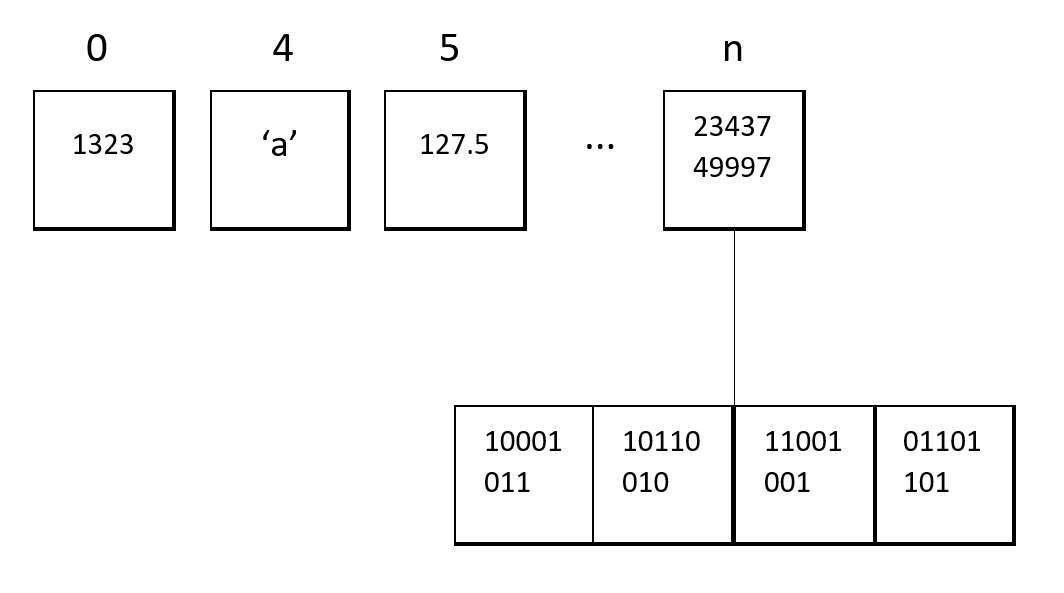
\includegraphics[scale=0.4]{Allocation.PNG}
  \caption{Memory Allocation of various data types}
  
\end{figure}
In Figure 1.1, the integer '1323' has taken 4 cubby holes or blocks sequentially from address '0' to '3'. Since a character is of 1 byte, character 'a' has taken only one cubby hole of address '4'.  The integer '234749997' has taken 4 cubby holes. Each cubby hole is of 8 bits or 1 byte. Therefore the binary representation of the integer is stored sequentially in the cubby holes. 

\subsection{Conditional statements}
Conditional statements are used to make decisions based on a given condition.\\
\begin{figure}[H]
  \centering
  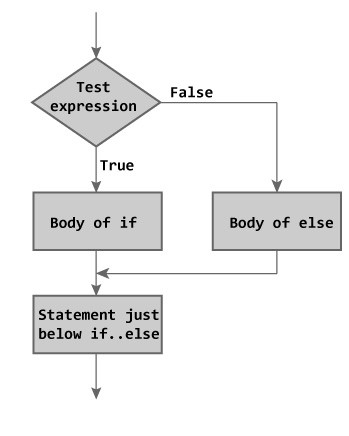
\includegraphics[scale=0.75]{if-else.jpg}
  \caption{Flowchart for if-else conditionals}
\end{figure}
~\\
\paragraph{Comparison operators with truth value}
Conditional statements work on the basis of the truth value of the expression used.
There are multiple comparison operators which return a truth value in boolean and are listed below. \\
\begin{table}[ht]
  \centering
  \begin{tabular}{|c|c|c|}
    \hline
    \thead{Operator} & \thead{Description} & \thead{Usage Example}\\
    \hline
    $==$ & equal to & \makecell{$1==1 \rightarrow$ true\\ 't' $==$ 'p' $\rightarrow$ false} \\
    \hline
    $!=$ & not equal to & \makecell{$5 != 5 \rightarrow$ false \\ $4.6 != 6.7 \rightarrow$ true }\\
    \hline
    $<$ & less than & \makecell{$5<4 \rightarrow$ false \\ 'a' $<$ 'b' $\rightarrow$ true ( using ASCII value)}\\
    \hline
    $<=$ & less than or equal to & \makecell{$4.5 <= 4.5 \rightarrow$ true \\ $3 <= 5.7 \rightarrow$ true }\\
    \hline
    $>=$& greater than or equal to & \makecell{'b' $>=$ 'b' $\rightarrow$ true \\ 
    true $>=$ false $\rightarrow$ true} \\
    \hline
    
  \end{tabular}
  \caption{Comparison operators}
  \label{tab:ComparisonOperators}
  
\end{table}
\begin{remark}
  Do not get confused between the assignment operator and equal to operator when using in an if-else conditional statement
\end{remark}

The example below shows the usage of if-else conditionals and comparison operators.
\begin{example}
  
  \begin{lstlisting}[language=C++, caption = Using if condition to check if number is divisible by 2]
    
    #include <iostream>
    using namespace std;
    int main()
    {
      int num; //variable to store input
      cout<<"Enter number: "<<endl; //To show prompt
      cin>>num; //Taking and storing input value
      if(num % 2 == 0) //"a%b" to check the remainder 
      {
        cout<<"Number is divisible by 2"<<endl;
      }
      else
      {
        cout<<"Number is not divisible by 2"<<endl;
      }
      return 0;
    }
  \end{lstlisting}
\end{example}
\subsection{Loops}
In a Loop construct a sequence of instructions are repeated till a specific condition or target is reached. ~\\ ~\\
There are three types of loops in C++: 
\paragraph{While loop}
A while loop statement repeatedly executes a target statement as long as a given condition is true. ~\\
The syntax of a while loop in C++ is:
\begin{lstlisting}
  while (testExpression) 
  {
    statement(s);
  }
\end{lstlisting}
where, \textbf{testExpression} is checked on each entry of the while loop.
~\\ \\
Here is the flow of control in a while loop: \\
\begin{itemize}
\item The while loop evaluates the \textbf{test expression}.
  If the \textbf{test expression} is true, code inside the body of while loop is evaluated.
\item Then, the \textbf{test expression} is evaluated again. This process goes on until the \textbf{test expression} is false.
\item When the \textbf{test expression} is false, while loop is terminated.
\end{itemize}
\begin{figure}[H]
  \centering
  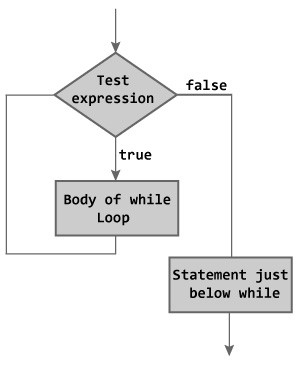
\includegraphics[scale=0.75]{while-loop.jpg}
  \caption{Flowchart of while loop}
\end{figure}
\begin{example}
  \begin{lstlisting}[language=C++, caption = Using While loop to increment an integer 5 times]
    
    #include <iostream>
    int main()
    {
      int num = 1; //variable to be incremented
      int count = 0; //to keep track of number of iterations
      while(count < 5)
      {
        num = num + 1; //or num++ can also be used to increment
        count++;
      }
      return 0;
    }
  \end{lstlisting}
\end{example}
\paragraph{Do-while loop}
The syntax of do-while loop is:
\begin{lstlisting}
  do {
    // codes;
  }
  while (testExpression);
\end{lstlisting}
Here is the flow of control in a while loop:
\begin{itemize}
\item The codes inside the body of loop is executed at least once. The \textbf{test expression} is checked.
\item If the \textbf{test expression} is true, the body of loop is executed. This process continues till the \textbf{test expression} becomes false.
\item When the \textbf{test expression} is false, do-while loop is terminated.
\end{itemize}
\begin{figure}[H]
  \centering
  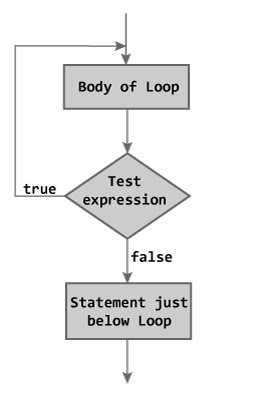
\includegraphics[scale=0.75]{dowhile-loop.jpg}
  \caption{Flowchart of do-while loop}
\end{figure}
\begin{example}
  \begin{lstlisting}[language=C++, caption = Using Do-While loop to increment an integer 5 times]
    
    #include <iostream>
    int main()
    {
      int num = 1; //variable to be incremented
      int count = 0; //to keep track of number of iterations
      do
      {
        num = num + 1; //or num++ can also be used to increment
        count++;
      }
      while(count<5)
      return 0;
    }
  \end{lstlisting}
\end{example}
\paragraph{For loop}
A for loop allows you to efficiently write a loop that needs to execute a specific number of times. ~\\
The syntax of a for loop is:
\begin{lstlisting}
  for(initializationStatement; testExpression; updateStatement) 
  {
    statement(s); 
  }
\end{lstlisting}
Here is the flow of control in a for loop:
\begin{itemize}
\item The \textbf{initialization statement} is executed only once at the beginning.
\item Then, the \textbf{test expression} is evaluated.
  If the \textbf{test expression} is false, for loop is terminated. But if the \textbf{test expression} is true, code inside body of for-loop is executed followed by the \textbf{update statement}.
\item Again, the \textbf{test expression} is evaluated and this process repeats until the \textbf{test expression} is false.
\end{itemize}
\begin{figure}[H]
  \centering
  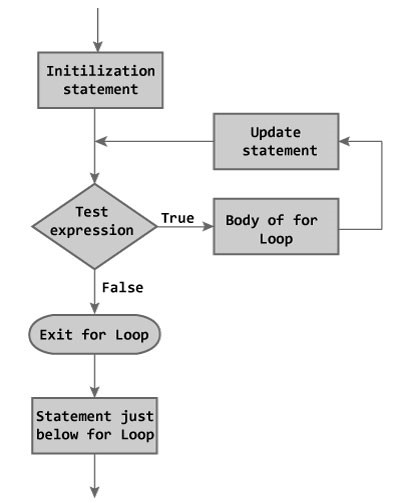
\includegraphics[scale=0.75]{for-loop.jpg}
  \caption{Flowchart of for loop}
\end{figure}
\begin{example}
  \begin{lstlisting}[language=C++, caption = Using For loop to increment an integer 5 times]
    
    #include <iostream>
    int main()
    {
      int num = 1; //variable to be incremented
      for(int i = 0; i < 5; i++)
      {
        num = num + 1; //or num++ can also be used to increment
      }
      return 0;
    }
  \end{lstlisting}
\end{example}

\begin{example}
  \begin{lstlisting}[language=C++, caption = Using While loop to increment an integer 5 times]
    #include <iostream>
    int main()
    {
      int num = 1; //variable to be incremented
      int count = 0; //to keep track of number of iterations
      while(count < 5)
      {
        num = num + 1; //or num++ can also be used to increment
        count++;
      }
      return 0;
    }
  \end{lstlisting}
\end{example}

\subsection{Functions}
A function is a group of statements that together perform a task. Every C++ program has at least one function which is main() but we can define additional functions as well.\\ ~\\ 
You can divide up your code into separate functions; how you divide up your code among different functions is up to you, but logically the division usually is such that each function performs a specific task. ~\\ ~\\
A function declaration tells the compiler about a function's name, return type, and parameters. A function definition provides the actual body of the function.
\paragraph{Defining a Function}
The general form of a C++ function definition is as follows:
\begin{lstlisting}
  return_type function_name( parameter1, parameter2, parameter3,... ) 
  {
    body of the function
  }
\end{lstlisting} ~\\ ~\\
A C++ function definition consists of a function header and a function body. Here are all the parts of a function: ~\\
\begin{itemize}
\item \textbf{Return Type} - A function may return a value. The return\textunderscore type is the data type of the value the function returns. Some functions perform the desired operations without returning a value. In this case, the return\textunderscore type is the keyword \textbf{void}. \\
\item \textbf{Function Name} - This is the actual name of the function. The function name and the parameter list, together constitute the function signature.\\
\item \textbf{Parameters} - A parameter is like a placeholder. When a function is invoked, you pass a value to the parameter. This value is referred to as actual parameter or argument. The parameter list refers to the type, order, and number of the parameters of a function. Parameters are optional; that is, a function may contain no parameters.\\
\item \textbf{Function Body} - The function body contains a collection of statements that define what the function does. ~\\
\end{itemize}

\paragraph{Declaring a function}
A function declaration tells the compiler about a function name and how to call the function. The actual body of the function can be defined separately.\\
\begin{lstlisting}
  return_type function_name( parameter list );
\end{lstlisting}
\newpage
\paragraph{Calling a function}
While creating a C++ function, you give a definition of what the function has to do. To use a function, you will have to call or invoke that function. \\ ~\\
When a program calls a function, program control is transferred to the called function. A called function performs defined task and when its return statement is executed or when its function-ending closing brace is reached, it returns program control back to the main function. \\ ~\\
To call a function, you simply need to pass the required parameters along with function nam, and if function returns a value, then you can store returned value.\\

\begin{example}
  \begin{lstlisting}[language=C++, caption = Declaration Definition and Calling of a max function]
    
    #include <iostream>
    using namespace std;
    
    // function declaration
    int max(int num1, int num2);
    
    int main () 
    {
      // local variable declaration:
      int a = 100;
      int b = 200;
      int ret;
      
      // calling a function to get max value.
      ret = max(a, b);
      cout << "Max value is : " << ret << endl;
      
      return 0;
    }
    
    // function returning the max between two numbers
    int max(int num1, int num2) 
    {
      // local variable declaration
      int result;
      
      if (num1 > num2)
      result = num1;
      else
      result = num2;
      
      return result; 
    }
  \end{lstlisting}
\end{example}

\newpage
\section{Problems}\index{Problems}
\begin{problem}
  
  A certain grade of steel is graded according to the following conditions: ~\\
  \begin{itemize}
    \setlength\itemsep{1em}
  \item Hardness must be greater than 50
  \item Carbon content must be less than 0.7 \item Tensile strength must be greater than 5600
  \end{itemize}
  ~\\ The grades are as follows: ~\\
  \begin{itemize}
    \setlength\itemsep{1em}
  \item Grade is 10 if all three conditions are met \item Grade is 9 if conditions (i) and (ii) are met
  \item Grade is 8 if conditions (ii) and (iii) are met 
  \item Grade is 7 if conditions (i) and (iii) are met
  \item Grade is 6 if only one condition is met
  \item Grade is 5 if none of the conditions are met
  \end{itemize}
  ~\\Write a program, which will require the user to give values of hardness, carbon content and tensile strength of the steel under consideration and output the grade of the steel.
  \paragraph{Instructions}
  \begin{itemize}
  \item Use if-else conditional statements 
  \end{itemize}
\end{problem}
~\\
\newpage
\begin{problem}
  Two frogs named 'FrogPrime' and 'Frogatron' are in a well of depth 1000 feet. They decide to race each other to the top to see who is the winner.~\\ ~\\
  Both frogs can jump 4 feet at a time but slide down 1 foot every time, thus making the total distance covered to be 3 feet. ~\\ \\
  FrogPrime has a 2 \% chance to get an adrenaline rush and jump 5 feet.
  Frogatron has special claws that have a 2\% chance to grab on to a wall, thus it does not slide down 1 foot if the claws connect ~\\ \\
  The frogs will keep on jumping till one of them clears the well and is declared a winner. ~\\ \\
  Your program should simulate this behavior. It should find out the winner and report it. It should also report if there is a tie. ~\\ \\
  It should also display the progress of the frogs at every 50th jump.~\\ \\
  It should also display the total number of jumps once the competition is over. ~\\ \\
  The output should be similar to this:\\ \\
  \begin{center}
    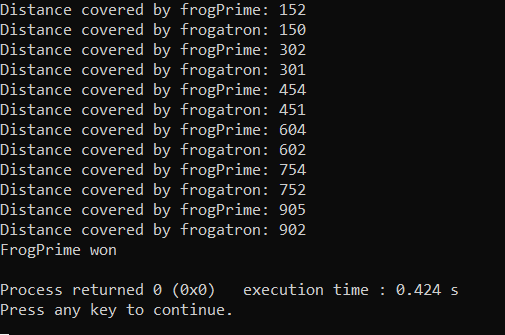
\includegraphics[scale=0.75]{Problem1_2.png}
  \end{center}
  \paragraph{Instructions}
  \begin{itemize}
  \item You can use random number generation to simulate chances. Find out yourself about using random number generation and ranges.
  \item Think in terms of loops and if-else conditionals
  \end{itemize}	
  
\end{problem} ~\\ 
\begin{problem}
  Write a function IsPrime(int n) to test whether a parameter is prime. Apply the function in a program which prints all the prime numbers up to 100.
  \paragraph{Instructions}
  \begin{itemize}
  \item Use modulo operator to check divisibility
  \item You can use bool to keep check if a number is prime
  \item Break the question in parts and work on the function first
  \end{itemize}
\end{problem}
~\\
\begin{problem}
  Write a function Fibonacci(int n) which calculates the nth Fibonacci number. Write a main program that uses this function and the function from Problem 1.3 to print out the first 5 Fibonacci numbers that are also primes.
  \paragraph{Instructions}
  \begin{itemize}
  \item Think in terms of loops and an extensive use of variables to keep track of the needed terms in every iteration
  \end{itemize}
\end{problem}

\newpage
\section{Solution}
\begin{lstlisting}[language=C++]
  // ... copy and paste your code
\end{lstlisting}

\newpage
\section{Student Feedback}
\textbf{What did you learn from this lab?}\\ 
\framebox(400,150){}\\
\textbf{What part of the lab is still unclear to you?}\\
\framebox(400,150){}\\
\textbf{What can be improved in this lab?}\\ 
\framebox(400,150){}
\newpage
% ----------------------------------------------------------------------------------------
\chapterimage{chapter_head_2.pdf} % Chapter heading image
\chapter{Pointers \hspace{60mm} {\textsc{\small SCRIPTED BY : ABDUL RAFAY MEHBOOB}}}
\section{Memory Address}\index{Paragraphs of Text}

As explained in the first lab, variables are stored into Random Access Memory (RAM) which is divided into chunks of memory space. Each chunk of memory has a unique address which is used to access the value stored in that particular memory location as shown in figure below:

% \begin{figure}[h]
%   \centering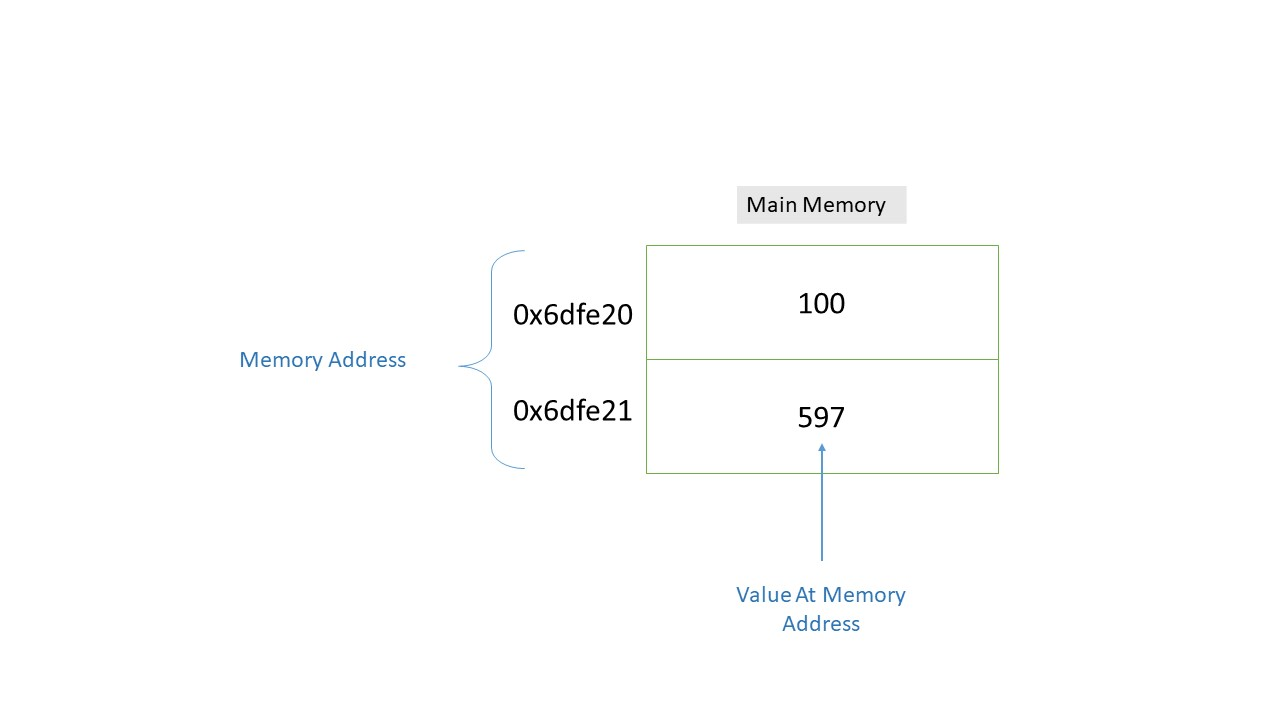
\includegraphics[scale=0.5]{ma.jpg}
%   \caption{Memory Address}
% \end{figure}

\subsection{Referencing by Address-of Operator}\index{Address-of Operator}
In C++ we have access to these memory locations by a special operator as describe in Figure 2.

\begin{figure}[h]
  \centering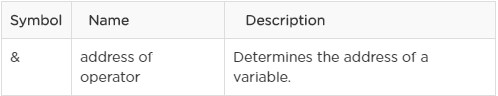
\includegraphics[scale=1]{addressOperator.jpg}
  \caption{Address-of Operator}
\end{figure}

\begin{lstlisting}[language=C++, caption = Address of a variable]
  void main()
  {
    int a = 10;
    cout << &a << endl;  //prints address of a
    cout << a << endl; // prints value of a 
  }
\end{lstlisting}
\textbf{Output:}
\begin{lstlisting}
  0x6dfefc 
  10
\end{lstlisting}

\begin{figure}[h]
  \centering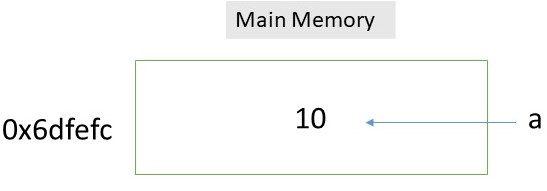
\includegraphics[scale=0.5]{addofex.jpg}
  \caption{Memory location of variable 'a'}
\end{figure} 
In programming, we will be requiring memory location of a variable frequently; hence it is convenient for programmers to store it in a variable and access it throughout the program if it is required. This storing of memory location of a variable into another variable is where we will introduce the concept of pointers. 
\section{Pointers}\index{Pointers}
\begin{definition}[Pointer] It is a variable used to store memory address of another variable
\end{definition}
\begin{lstlisting}[language=C++, caption = Pointer variable]
  int a = 100;
  int* pointer_variable; //declaration of pointer variable
  pointer_variable = &a; //assigning address of 'a' to the pointer variable

  cout << a << endl;
  cout << pointer_variable << endl;

\end{lstlisting}
\textbf{Output:} 
\begin{lstlisting}
  100
  0x6dfefc
\end{lstlisting}

\begin{tcolorbox}[width=\textwidth,colback={white},title={KEYNOTE},colbacktitle=purple!50!white,coltitle=black]    
  Please note that only address of a variable should be assigned to a pointer. \emph{If a value of a variable is assigned to a pointer} then the program will crash or show error.

  \begin{lstlisting}[language=C++, caption = Incorrect initialization of a pointer]
    int a = 3;
    int* ptr = a; //program will crash at this point
  \end{lstlisting}
  
  \hfill \break
  There are multiple ways to declare a pointer:
  \begin{enumerate}
  \item int *ptr;
  \item int * ptr;
  \item int* ptr;
  \end{enumerate}
  Even though all the methods are correct,it is a common coding practice to use third way of declaration.
\end{tcolorbox}

\hfill \break
In principle, pointers are meant to point to a valid address, such as the address of a variable. However, pointers can point to any address in the memory including the address that do not refer to any valid element or variable. An example of that is an uninitialized pointer. In this case pointer is pointing to a \emph{garbage value}. \\

\begin{definition}[Garbage Value]
  When a variable is declared but not initialized, the block of memory that has been allocated to variable still contains some value that has been left over from previous programs and operations. That value is called garbage value and it may lead to error in program
\end{definition}


\begin{lstlisting}[language=C++, caption = Un-initialize pointer]
  int* ptr; //uninitialized pointer
  cout << ptr; //prints invalid address of main memory
\end{lstlisting}
\textbf{Output:}
\begin{lstlisting}
  0x427020 
\end{lstlisting}


\hfill \break
However, in some cases pointer is explicitly required to point nowhere. For such cases, there exists a special value that any pointer type can take: the null pointer value. This value can be expressed in three ways:
\begin{enumerate}
\item int* ptr = 0;
\item int* ptr = nullptr;
\item int* ptr = NULL;
\end{enumerate}

\subsection{Dereferencing}
Dereferencing a pointer means getting the value stored in the memory location pointed by the pointer.
We use dereferencing operator(also known as indirection operator as described in Figure 4) to get the 'value pointed by' a pointer.
\begin{figure}[h]
  \centering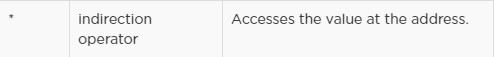
\includegraphics[scale=1]{indirect.jpg}
  \caption{Indirection Operator}
\end{figure} \\ \\ \\

\begin{lstlisting}[language=C++, caption = Dereferencing a pointer]
  int a = 10;
  int* ptr = &a; 
  cout << ptr << endl;
  cout << *ptr << endl; 
\end{lstlisting}
\textbf{Output:}
\begin{lstlisting}
  0x427020
  10
\end{lstlisting}

\begin{tcolorbox}[width=\textwidth,colback={white},title={KEYNOTE},colbacktitle=purple!50!white,coltitle=black] 
  The asterisk (*) sign in the declaration of the pointer does not mean “value pointed by”, it only means that it is a pointer. It should not be confused with the dereference operator. They are simply two different things represented with the same sign.
\end{tcolorbox}
\hfill \break
Since pointer can access the value pointed by the pointer, changes can be made in this value directly through pointer.
\begin{lstlisting}[language=C++, caption = Modifying value of the address pointed by the pointer]
  int a = 10;
  int* ptr = &a; 
  cout << *ptr << endl;
  cout << a << endl;

  *ptr = 7;  // value pointed by pointer is now changed
  cout << *ptr << endl;
  cout << a << endl;  // value of a is changed to 7 as well
\end{lstlisting}
\textbf{Output:} 
\begin{lstlisting}
  10
  10
  7
  7
\end{lstlisting}

\begin{example}
  \begin{lstlisting}[language=C++, caption = Understanding Reference]

    void UnderstandingReferences()
    {
      int val = 50;
      int& ref_val = val;
      
      ref_val = 100;
      
      cout<<val<<endl;
    }
    int main()
    {
      UnderstandingReferences();	
    }
  \end{lstlisting}
\end{example}

\begin{example}
  \begin{lstlisting}[language=C++, caption = Understanding Pointers]

    void UnderstandingPointers();
    int val = 10;
    int* ptr_val = NULL;//Pointer is assing NULL so it points nowhere
    
    cout<<val<<endl;
    cout<<ptr_val<<endl;
    
    ptr_val = &val;//Giving the address of 'val' to the pointer
    
    cout<<val<<endl; //Outputting the stored value
    cout<<ptr_val<<endl; //Outputting the LVALUE of variable 'val'
    cout<<*ptr_val<<endl; //Outputting the RVALUE of variable 'val'
    
    *ptr_val = 20;
    
    cout<<val<<endl;        //Outputting vals value which is changed 
    cout<<ptr_val<<endl;    //Outputting the LVALUE of variable 'val'
    cout<<*ptr_val<<endl;   //Outputting the RVALUE of variable 'val'

    int main()
    {
      UnderstandingPointers();
      return 0;
    }
  \end{lstlisting} 
  \textbf{Output:}
  \begin{lstlisting}
    10
    0
    10
    0x6dfef8
    10
    20
    0x6dfef8
    20
  \end{lstlisting}

\end{example}

\section{Passing Value}
There are multiple ways in which parameter data can be passed into and out of a function. We will study following methods in this course:
\begin{enumerate}
\item Pass by Value
\item Pass by Reference
\item Pass by Pointer
\end{enumerate}
\subsection{Pass by Value}
In this method, a copy of the argument is passed to the function. This copy is destroyed as the program exceeds the scope of the function.
\begin{lstlisting}[language=C++, caption = Pass by value]
  void PassByValue(int x)
  {
    cout << (x+1) << endl;
  }
  int main()
  {
    int y = 5;
    PassByValue(y); \\First call
    PassByValue(y+1); \\Second call
    PassByValue(y+2); \\Third call
    
    cout << y << endl;
    
    return 0;
  }
\end{lstlisting}
\textbf{Output:}
\begin{lstlisting}
  6
  7
  8
  5
\end{lstlisting}

\begin{tcolorbox}[width=\textwidth,colback={white},title={KEYNOTE},colbacktitle=purple!50!white,coltitle=black]  
  Since a copy of argument is passed to the function, the original argument can not be modified by the function as shown above.
\end{tcolorbox}
\hfil \break
\textbf{Advantages of passing by value}\\
Arguments passed by value can be variables (e.g. x), literals (e.g. 6), expressions (e.g. x+1), structs and classes, and enumerators. In other words, just about anything.
Arguments are never changed by the function being called, which prevents side effects.\\
\textbf{Disadvantages of passing by value} \\
Copying structs and classes can incur a significant performance penalty, especially if the function is called many times.\\
\textbf{When to use pass by value}\\
When passing fundamental data type and enumerators, and the function does not need to change the argument.\\
\textbf{When not to use pass by value}\\
When passing arrays, structs, or classes.\\ \\
In most cases, pass by value is the best way to accept parameters of fundamental types when the function does not need to change the argument. Pass by value is flexible and safe, and in the case of fundamental types, efficient

\subsection{Pass by Reference}
In this method, reference to an argument is passed to the function. Since reference to a variable is treated exactly the same way as the variable itself, any changes made to the reference is passed onto the argument. To pass a variable by reference we modify the function parameter as reference.\\
\begin{lstlisting}[language=C++, caption = Pass by reference]
  void PassByReference(int &x)
  {
    x = 777; 
  }
  int main()
  {
    int y = 5;
    PassByReference(y); 
    cout << y << endl;
    
    return 0;
  }
\end{lstlisting}
\textbf{Output:} 
\begin{lstlisting}
  777
\end{lstlisting}
\textbf{Advantages of passing by reference}\\
References allow a function to change the value of the argument, which is sometimes useful.A copy of the argument is not made,therefore,this method is fast, even when used with large structs or classes.
References can be used to return multiple values from a function.\\
\textbf{Disadvantages of passing by reference}\\
It’s impossible to tell from the function call whether the argument may change.\\
\textbf{When to use pass by reference}\\
When passing structs or classes.
When you need the function to modify an argument.
When you need access to the type information of a fixed array.\\
\textbf{When not to use pass by reference}\\
When passing fundamental types that don’t need to be modified (use pass by value)
\subsection{Pass by Address}
This method involved passing address of argument variable rather than the variable itself. Pointer are used to store this address as function parameter and then this pointer is dereferenced to access or change the value. This method is mostly used to pass an array to a function.

\begin{lstlisting}[language=C++, caption = Pass by Address]
  void PassByPointer(int* x)
  {
    x = x+1; 
  }
  int main()
  {
    int y = 5;
    PassByPointer(&y); 
    cout << y << endl;
    
    return 0;
  }
\end{lstlisting} 
\textbf{Output:} 
\begin{lstlisting}
  6
\end{lstlisting}
\textbf{Advantages of passing by address}\\
Pass by address allows a function to change the value of the argument, which is sometimes useful. .
In this method, a copy of the argument is not made ,therefore,it is fast even when used with large structs or classes.
It is possible return multiple values from a function using this method.\\
\textbf{Disadvantages of passing by address}\\
Since literals and expressions do not have addresses, pointer arguments must be normal variables.
All values must be checked to see whether they are null.\\
\textbf{When to use pass by address}\\
When passing arrays.When passing a pointer\\
\textbf{When not to use pass by address}\\
When passing structs or classes.When passing fundamental types

\subsection{Dynamic Memory Allocation}
You can declare memory dynamically using a pointer. Once you no longer require that memory location, you deallocate it. As a result, the memory consumption of a program might change during its execution. If you forget to deallocate memory, the memory stays assigned even when the program finishes thus resulting in a memory leak.
\begin{lstlisting}
  int* ptr = new int;
  *ptr = 100;
  cout<<*ptr;
  delete ptr;
  ptr = nullptr;
\end{lstlisting}

\section{Structures}
The struct keyword defines a structure type followed by an identifier (name of the structure). Then inside the curly braces, you can declare one or more members (declare variables inside curly braces) of that structure. For example:
\begin{lstlisting}
  struct Light
  {
    int brightness;
    bool activated;
  };
\end{lstlisting}
Here a structure light is defined which has two members: brightness and activated. When a structure is created, no memory is allocated. The structure definition is only the blueprint for the creating of variables. You can imagine it as a datatype. You can define functions within a structure to control the attributes within the structure.
\begin{lstlisting}
  struct Light
  {
    int brightness;
    bool activated;
    
    void Brighten()
    {
      brightness++;
    }
  };
\end{lstlisting}

\section{Problems}


\begin{problem}
  Write 3 versions of a {\tt swap} function as follows.
  \begin{itemize}
  \item one that calls by value.
  \item one that calls by reference.
  \item one that calls by pointer/address.
  \end{itemize}
\end{problem}

\begin{problem}
  Write a function that asks the user to enter integers as inputs to be stored in the variables {\tt a} and {\tt b} respectively. There are also two integer pointers named {\tt ptrA} and {\tt ptrB}. Assign the addresses of {\tt a} and {\tt b} to {\tt ptrA} and {\tt ptrB} respectively, and display them.
\end{problem}

\begin{problem}
  Write a function to accept five integer values from keyboard. Store the values in an array using a pointer. Then print the elements of the array on the screen.
\end{problem}

\begin{problem}
  Write a function to find the max of an integral data set. The function will ask the user to input the number of data values in the set and each value. The program prints on screen a pointer that points to the max value.
\end{problem}

% \begin{problem}
%   A data center manager wants to write a program that turns on an alarm when temperature,pressure or humidity of the data center exceeds the maximum limit or decreases beyond the minimum limit.You are required to write a program that takes user input for this maximum and minimum values for temperature,pressure and humidity and controls the alarm based on the current conditions entered by the user. Code has been provided, you need to add your code where required.\\
% \end{problem}

% \hfill \break
% \textbf{Structure of Code}
% \begin{lstlisting}[language=C++, caption = Task]
%   bool checkTemp(int curr,int* tem);
%   void checkPes(int curr,int& max,int* min, bool& alar);
%   void checkHum(int curr,int* max,int* min, bool* alar);

%   int main()
%   {
%   int humdity[2] = {0,0};
%   int temp[2] = {0,0};
%   int press[2] = {0,0};
%   int current_reading[3] = {0,0,0};
%   bool alarm = false;

%   for (int i = 0;i<50;i ++)     //menu display
%   {
% 		cout<<"~";
% }
%   cout<<"\n WELCOME TO DATA CENTER \n";     //menu display
%   for (int i = 0;i<50;i ++)     //menu display
%   {
% 		cout<<"~";
% }
%   cout<<endl;
%   cout<<"Please enter maximum limit of temperature: ";
%   cin>>temp[0]; cout<<endl;
%   cout<<"Please enter minimum limit of temperature: ";
%   cin>>temp[1]; cout<<endl;

%   cout<<"Please enter maximum limit of pressure: ";
%   cin>>press[0]; cout<<endl;
%   cout<<"Please enter minimum limit of pressure: ";
%   cin>>press[1]; cout<<endl;	

%   cout<<"Please enter maximum limit of humidity: ";
%   cin>>humdity[0]; cout<<endl;
%   cout<<"Please enter minimum limit of humidity: ";
%   cin>>humdity[1]; cout<<endl;

%   system("CLS");
%   bool terminator = false;
%   char inp;
%   while (terminator != true)
%   {
% 		cout<<"Please enter current reading of temperature: ";
% 		cin>>current_reading[0]; cout<<endl;
% 		cout<<"Please enter current reading of pressure: ";
% 		cin>>current_reading[1];cout<<endl;
% 		cout<<"Please enter current reading of humidity: ";
% 		cin>>current_reading[2];cout<<endl;

% 		alarm = checkTemp(current_reading[0],temp);
% 		checkPes(current_reading[1],press[0],&press[1], alarm);
% 		checkHum(current_reading[2], &humdity[0], &humdity[1], &alarm);

% 		if (alarm == true)
% 		{
%   cout<<"Alarm is on"<<endl;
% }
% 		else
% 		{
%   cout<<"All is well"<<endl;
% }

% 		cout<<"enter 'c' to continue and 'e' to exit ";
% 		cin>>inp;cout<<endl;

% 		if (inp == 'e')
% 		{
%   terminator = true;
% }
% 		else if(inp == 'c')
% 		{
%   system("CLS");
% }
% 		else
% 		{
%   cout<<"You entered wrong input, program terminated"<<endl;
%   terminator = true;
% }
% }

%   return 0;
% }

%   bool checkTemp(int curr,int* tem)
%   {
%   //Write your code here
% }
%   void checkPes(int curr,int& max,int* min, bool& alar)
%   {
%   //Write your code here
% }
%   void checkHum(int curr,int* max,int* min, bool* alar)
%   {
%   //Write your code here
% }

% \end{lstlisting}
% ~\\
% \begin{problem}
%   Create 2 different integer arrays of different lengths.	Pass them to a function which defines a dynamic array that contains all the values of the passed arrays and then it returns the address of the dynamic array.\\
%   \paragraph{Instructions}
%   \begin{itemize}
% 		\item Do not forget to deallocate memory.
% 		\item You will need to pass the size of the arrays as well.
%   \end{itemize}
% \end{problem}
% ~\\
% \begin{problem}
%   Use a pointer to input and output values from an array like a stack.\\
%   \paragraph{Instructions}
%   \begin{itemize}
% 		\item You will need to understand pointer arithmetics to do this task.
%   \end{itemize}
% \end{problem}
% ~\\

% \begin{problem}
%   As required in the above problem, use a pointer to input and output values from an array like a stack but the array should be inside a structure named 'Stack'. Create another structure named 'Queue' and make it behave like a Queue. The pointers should be under the 'private' access specifier. Define appropriate functions for your structures\\
%   \paragraph{Instructions}
%   \begin{itemize}
% 		\item Since you will be using an array, it will have a fixed length.
% 		\item If you make the same with a dynamic array, what problem do you think might happen? try implement using a dynamic array and find out.
%   \end{itemize}
% \end{problem}

\newpage
\section{Solution}
\begin{lstlisting}[language=C++]
  // ... copy and paste your code
\end{lstlisting}

\newpage
\section{Student Feedback}
\textbf{What did you learn from this lab?}\\
\noindent\fbox{\parbox{\textwidth}{
    % Your feedback here.
  }
}\\
\textbf{What part of the lab is still unclear to you?}\\
\noindent\fbox{\parbox{\textwidth}{
    % Your feedback here.
  }
}\\
\textbf{What can be improved in this lab?}\\ 
\noindent\fbox{\parbox{\textwidth}{
    % Your feedback here.
  }
}

\newpage

% ----------------------------------------------------------------------------------------
\chapterimage{chapter_head_2.pdf} % Chapter heading image
\chapter{Classes \& Objects in C++ \hspace{14mm} {\textsc{\small SCRIPTED BY : NABIHA \& MINHAJ}}}

\section{Objective}\index{Objective}

This Lab session introduces you to the most fundamental concept in Object Oriented Programming, Classes and Objects.

\begin{itemize}
\item Understand the concept of Classes \& Objects in OOP.
\item Understand the concept and use of Data Members and Member Functions.
\item Understand Data Encapsulation and its use.
\item Learn to make a Class consisting of Data Members and Member Functions.
\item Use Classes to make Objects, and use these Objects in your Programs.
\end{itemize}
\section{Key Concepts}\index{Key Concepts}

\subsection{Objects}

In Programming, an Object is a collection of variables and functions that together serve as a unique entity. You can think of Objects in Programming like Real World Objects, having different properties and characteristics. Similarly, Objects in Programming have \textbf{Data Members} which define the state of the object and \textbf{Member Functions} which define the behavior of the object. The figure might help in understanding.Make, Model and Speed are the Properties of the Car which can be modeled as Data Members, and StartEngine(), MoveCar() and StopEngine() are the behaviors of the car, which can be modeled as Member Functions. Params are the parameters of the Member Functions. It depend on the function how many parameters are required. 

\begin{figure}[H]
  \centering
  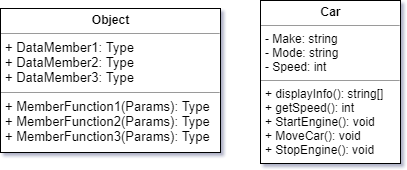
\includegraphics[scale=0.7]{Cars.png}
  \caption{Comparison of a Programming Object and Real World Object}
  \label{fig:my_label}
\end{figure}

\subsection{Data Members}

Objects contain variables that are unique to that Object. These variables are called \textbf{Data Members} (also known as \textbf{Attributes} or 
\textbf{Properties}). For example, a car may have model, make, color and registration number and other properties that are unique to it and may serve to identify it from other cars.

% https://www.cs.nmsu.edu/~rth/cs/cs177/map/datamem.html

\subsection{Member Functions}

Similar to how real world objects have certain properties, they also have certain behaviors, which may change their own properties or of other objects. For example, a car changes its state from rest to motion when it starts moving. Here, the movement of the car can be modeled as a function of the car, which changes the 'state' of the car from rest to motion.
In the context of programming, functions are defined inside classes, called \textbf{Member Functions} (also known as \textbf{Methods} and \textbf{Procedures}), which are used for various purposes for the objects. A Member Function may be associated with the object, or with the whole class of objects if it's static. 

\subsection{Class}

Classes are the templates, or the blueprints for Objects. They specify the Data Members and the Methods that are to be available to the object. A Class is a specification, and the Object is the realization of that specification.

\begin{figure}[ht]
  \centering
  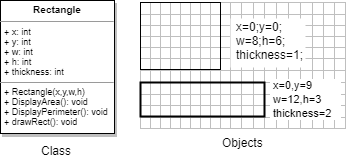
\includegraphics[scale = 0.88]{RectObject.png}
  \caption{Class Versus Objects}
  \label{fig:my_label}
\end{figure}

Objects are initialized from Classes, using \textbf{Constructors}, special member functions that are called for initialization of the Object. Constructors have the same name as the Class, and do not have a return type. They are used to assign default values to the Data Members of the Object being initialized. They can be overloaded like other functions with different parameters. If the Class doesn't have a constructor specified, the default constructor is called.

\subsection{Structure}

In C++, there are two types Classes, \textbf{Structs} and \textbf{Classes}. You can use either of the two keywords \texttt{struct} or \texttt{class} for making a Class. The only difference between them is that the default Access Specifier is Private for \texttt{class} and Public for \texttt{struct}. That means, if you don't specify an Access Specifier in your code, the Data Members and the Member Functions are automatically set to the default Access. Access Specifiers are discussed in the next topic.

\subsection{Encapsulation}

Encapsulation refers to the bundling of Data Members and Member Functions within one unit, i.e Objects. It also refers to the hiding of information to prevent interference from outside the Class, which may break the functionality of the code. For this reason, Classes have Private and Public Access Specifiers. Private Data Members and Member Functions can only be accessed within the class, while Public Data Members and Member Functions can be accessed from outside as well within the class. Usually, most Data Members are kept private, and are accessed from outside the class using special Member Functions called Getters and Setters. In C++, you can define Data Members and Functions inside the class without any Access Specifiers, which would mean that those Data Members and Functions will have the default Access Specifier.

\section{Syntax Examples}\index{Syntax Examples}

We will make a class Time using the keyword \texttt{struct} for Public Access to its Data Members.

\begin{lstlisting}[language=C++, caption=Class Definition using the \texttt{struct} keyword in C++]
  struct Rectangle
  {
    int x;      // Data Member 1
    int y;      // Data Member 2
    int width;  // Data Member 3
    int height; // Data Member 4
    // These Data Members are uninitialized,
    // and contain garbage values.
    
    void DisplayArea()      // Member Function 1
    {
      int area = width * height;
      cout << "Area of Rectangle = " << area << endl;
    }
    
    void DisplayPerimeter() // Member Function 2
    {
      int perimeter = 2 * (width + height);
      cout << "Perimeter of Rectangle = " << perimeter << endl;
    }
  }
\end{lstlisting}

Now, we create an object of Rectangle Class in our main() function. We will then initialize its Data Members and call its Member Functions.

\begin{lstlisting}[language=C++, caption=Making an Object using the Class and using its Data Members and Functions]
  int main()
  {
    Rectangle rect      // Making an object of type Rectangle
    rect.x = 0;         // Setting the values of the Data Members
    rect.y = 0;         // Data Members and Member Functions of an
    rect.width = 4;     // object are called by writing the name 
    rect.height = 6;    // of the object followed by a dot and the  
    rect.DisplayArea(); // name of the Member Function or Data Member
    rect.DisplayPerimeter();
  }
\end{lstlisting}

Here you see we made a Rectangle object and assigned values to its Data Members, and then output its area and perimeter on the console. Now, we might want to have default values for the Data Members of this Class. For that, we initialize the Data Members inside the class, so when we make our object, it has default values loaded in it. For that, we make the constructor of the Class.

\begin{lstlisting}[language=C++, caption={Default Class Constructor, to be defined inside the Class Body}]
  Rectangle()
  {
    x = 0;      // Initialize all Data Members
    y = 0;      // to default values for the 
    width = 0;  // member functions to work
    height = 0; // correctly
  }
\end{lstlisting}


We made a default constructor that initializes the Data Members to default values, but what if we want to initialize the object to values we provide, so we don't have to change its Data Members in the main() function everytime we create the object? For that we will make an overloaded constructor, which takes our values as arguments and assigns to the Data Members. An overloaded constructor is made in the same way as an overloaded function, but with no return type as it's a constructor.

\begin{lstlisting}[language=C++, caption={Overloaded Constructor, to be defined inside the Class Body}]
  Rectangle(int x1, int y1, int w, int h) // Overloaded Class  
  {                   // Constructor with Parameters.
    x = x1;             // Initialize all Data Members
    y = y1;             // to the input values for the 
    width = w;          // member functions to work
    height = h;         // correctly
  }
\end{lstlisting}

By providing the values in the arguments of the constructor, we can directly make an object with the desired values, and we won't have to change its Data Members in the main() function. This eases code maintenance.

In actual practice, Data Members are kept hidden from outside the class by making them Private, and are accessed using Member Functions called getters and setters. For that we use the \texttt{private} Access Specifier, and for allowing access from outside we use \texttt{public} Access Specifier. Since we were using \texttt{struct}, all data members and member functions were \texttt{public}.

\begin{lstlisting}[language=C++, caption=Class Definition using the \texttt{struct} keyword in C++]
  struct Rectangle
  {
    private:
    int x;                  // These Data Members are
    int y;                  // uninitialized, and contain
    int width;              // garbage values.
    int height;            
    public:
    Rectangle()             // Default Class Constructor
    {
      x = 0;              // Initialize all Data
      y = 0;              // Members to Default
      w = 0;              // Values.
      h = 0;
    }
    // Overloaded Class Constructor with Parameters
    Rectangle(int X, int Y, int W, int H)
    {
      x = X;              // Initialize all Data
      y = Y;              // Members to the given
      width = W;          // Values.
      height = H;
    }
    void DisplayArea()      // Calculate and Display Area
    {
      int area = width * height;
      cout << "Area of Rectangle = " << area << endl;
    }
    
    void DisplayPerimeter() // Calculate and Display Perimeter
    {
      int perimeter = 2 * (width + height);
      cout << "Perimeter of Rectangle = " << perimeter << endl;
    }
    void setX(int X)        // Member Function 3
    {
      x = X;
    }
    void setY(int Y)        // Member Function 4
    {
      y = Y;
    }
    void setW(int W)        // Member Function 5
    {
      width = W;
    }
    void setH(int H)        // Member Function 6
    {
      height = H;
    }
  }
\end{lstlisting}

It is not necessary to define the member function body inside the class. You can just declare the function prototype inside the class, and define it outside the class.

\begin{lstlisting}[language=C++, caption=Class Definition using the \texttt{struct} keyword in C++]
  struct Rectangle
  {
    private:
    int x;                   // Data Member 1
    int y;                   // Data Member 2
    int width;               // Data Member 3
    int height;              // Data Member 4
    public
    Rectangle();             // Default Constructor
    // Overload Constructor
    Rectangle(int x1, int y1, int w, int h);
    void DisplayArea();      // Member Function 1
    void DisplayPerimeter(); // Member Function 2
    void setX(int X);
    void setY(int Y);
    void setW(int W);
    void setH(int H);
  }
\end{lstlisting}

And then, we use the \textbf{Scope Resolution Operator} in order to define the bodies of member functions outside their respective classes. The next example will show how to define member functions outside the class.

\begin{lstlisting}[language=C++, caption=Class Definition using the \texttt{struct} keyword in C++]
  void Rectangle::DisplayArea()     // Calculate and Display Area
  {
    int area = width * height;
    cout << "Area of Rectangle = " << area << endl;
  }
  void Rectangle::DisplayPerimeter()// Calculate and Display Perimeter
  {
    int perimeter = 2 * (width + height);
    cout << "Perimeter of Rectangle = " << perimeter << endl;
  }
  void Rectangle::setX(int X)       // Set the x coordinate
  {
    x = X;
  }
  void Rectangle::setY(int Y)       // Set the y coordinate
  {
    y = Y;
  }
  void Rectangle::setW(int W)       // Set the width
  {
    width = W;
  }
  void Rectangle::setH(int H)       // Set the height
  {
    height = H;
  }
\end{lstlisting}

In practical situations, the class definition and the declarations of the member functions are written in one file called the header file having a \texttt{.h} extension, and the definition of the member functions including the constructors is made in another file called the source file, having a \texttt{.cpp} extension. This allows ease for maintaining, managing and reusing the code. We include the header file in the source file using the \texttt{\#include} directive, and then where we want to use our class, we simply include the header file into our main working file.

\newpage
\section{Problems}\index{Problems}

\begin{problem} Make a calculator that performs the four basic arithmetic operations on Complex Numbers. The program should ask for the real and imaginary part of the numbers, perform the desired operations and then output the real and imaginary parts of the operation.\\
\end{problem} 

\begin{problem} Write a C++ Class called Student, that takes the name, roll number and marks for five subjects. Also make Member Functions to display student info, display marks, percentage and total marks.\\
\end{problem}

\begin{problem} Write a C++ Class called Trucks that takes input from a file of different entries and puts them into an array of Truck Objects. The Entries include Driver's Name, Truck Registration Number, Fuel, Loaded Weight.
\end{problem}

\newpage
\section{Solution}
\begin{lstlisting}[language=C++]
  // ... copy and paste your code
\end{lstlisting}

\newpage
\section{Student Feedback}\index{Student Feedback}
\textbf{What did you learn from this lab?}\\
\noindent\fbox{\parbox{\textwidth}{
    % Your feedback here.
  }
}\\
\textbf{What part of the lab is still unclear to you?}\\
\noindent\fbox{\parbox{\textwidth}{
    % Your feedback here.
  }
}\\
\textbf{What can be improved in this lab?}\\ 
\noindent\fbox{\parbox{\textwidth}{
    % Your feedback here.
  }
}

\newpage
\chapterimage{chapter_head_2.pdf} % Chapter heading image
\chapter{Stacks \hspace{76mm} {\textsc{\small SCRIPTED BY : HAMZA MASROOR}}}
\section{Objective}\index{Objective}
In this lab, we'll learn about a data structure, called Stack. We'll learn about its implementation, operations and uses.
\section{Description}\index{Description}
Stack is a linear data structure which follows a particular order in which the operations are performed. The order may be LIFO (Last In First Out) or FILO (First In Last Out).\\ ~\\
Mainly the following three basic operations are performed in the stack:
\begin{itemize}
\item \textbf{Push}: Adds an item in the stack. If the stack is full, then it is said to be an Overflow condition.
\item \textbf{Pop}: Removes an item from the stack. The items are popped in the reversed order in which they are pushed. If the stack is empty, then it is said to be an Underflow condition.
\item \textbf{Peek or Top}: Returns top element of stack.
\item \textbf{isEmpty}: Returns true if stack is empty, else false.
\end{itemize}
\begin{figure}[H]
  \centering
  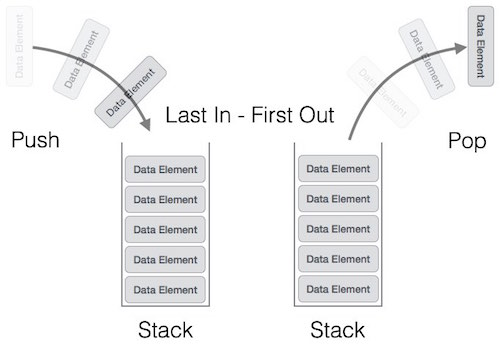
\includegraphics[scale=0.3]{stack.jpg}
  \caption{Representation of stack}
\end{figure}
\newpage
\subsection{Real-life example of stack}
There are many real life examples of stack. Consider the simple example of plates stacked over one another in canteen. The plate which is at the top is the first one to be removed, i.e. the plate which has been placed at the bottommost position remains in the stack for the longest period of time. So, it can be simply seen to follow LIFO/FILO order.
\subsection{Time Complexities of operations on stack}
push(), pop(), isEmpty() and peek() all take O(1) time. We do not run any loop in any of these operations.

\subsection{Applications of stack}
There are many possible applications of stack. Some are listed below:
\begin{itemize}
\item Balancing of symbols
\item Infix to Postfix /Prefix conversion
\item Redo-undo features at many places like editors, photoshop.
\item Forward and backward feature in web browsers
\item Used in many algorithms like Tower of Hanoi, tree traversals, stock span problem, histogram problem.
\item Other applications can be Backtracking, Knight tour problem, rat in a maze, N queen problem and sudoku solver
\end{itemize}
\subsection{Implementation}\index{Implementation}
We will be implementing a linked list based stack. In a linked list based stack, we have nodes linked to each other.
Each node stores a data and a link to the node next to it.
\begin{figure}[H]
  \centering
  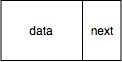
\includegraphics{node.jpg}
  \caption{Representation of node}
\end{figure}
\paragraph{Implementing Node}
To implement node, we will be making a struct to hold data and the link. In this implementation we are making a node to store integer type data. However, it can be implemented to store any data type or object.
\begin{lstlisting}
  struct Node
  {
    int data; \\To store data
    Node* next; \\To store the address or link to the next node
  };
\end{lstlisting}
\newpage
\paragraph{Initializing the Stack}
As a stack consists of many nodes, we should have many nodes inside our stack class, but we will have only one node, "head", which will act as a reference node and allows us to iterate through all the nodes till the end of the stack.

\begin{lstlisting}
  class Stack
  {
    private:
    Node* head;
    
    public:
    Stack()
    {
      head = NULL;
    }
  };		

\end{lstlisting}
Our stack now consists of a Node pointer which will hold the address of the head (i.e the top element) of the stack. To initialize, it is set to \textbf{NULL}, as the stack is empty.
\begin{figure}[H]
  \centering
  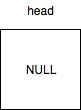
\includegraphics{head.jpg}
  \caption{Stack's head pointer}
\end{figure}

\paragraph{Implementing Push() operation}
Inside the class of Stack, we will declare and define a function "Push(int val)" in public.
\begin{lstlisting}
  void Push(int val)
  {
    if (head == NULL)
    {
      head = new Node;
      head->data = val;
      head->next = NULL;
    }
    else
    {
      Node* temp = head;
      head = new Node;
      head->data = val;
      head->next = temp;
    }
  }
\end{lstlisting}
\newpage
\begin{example}
  Let's visualize an example Push() operation\\
  \begin{lstlisting}
    Stack stack;
    stack.Push(5);
  \end{lstlisting}
  Since the stack is empty and head is set to NULL. Body of 'if' will be executed.\\
  It first creates a new node\\
  \begin{figure}[H]
    \centering
    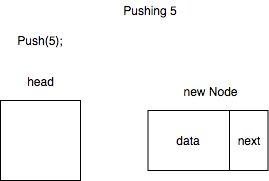
\includegraphics[scale=0.5]{push(1).jpeg}
    \caption{Creating new node for Push(5)}
  \end{figure}
  ~\\
  Then it sets head pointer to the new node.
  \begin{figure}[H]
    \centering
    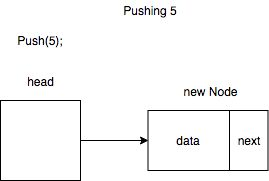
\includegraphics[scale=0.5]{push(2).jpeg}
    \caption{Setting head pointer}
  \end{figure}
  ~\\
  Then it sets the data and next pointer of new node.
  \begin{figure}[H]
    \centering
    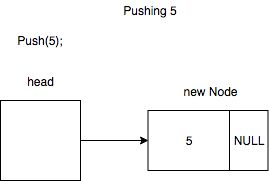
\includegraphics[scale=0.5]{push(3).jpeg}
    \caption{Setting data and next pointer}
  \end{figure}
\end{example}
\newpage
Since, head is not \textbf{NULL}, Push operation will now execute body of 'else'. Let's see an example
\begin{example}
  \begin{lstlisting}

    stack.Push(3);
  \end{lstlisting}
  It will first create a temporary node pointer, temp.
  \begin{figure}[H]
    \centering
    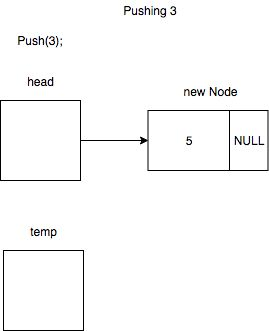
\includegraphics[scale=0.5]{push(4).jpeg}
    \caption{Creating temp pointer}
  \end{figure} ~\\
  Then it sets the temp to the node where head is pointing
  \begin{figure}[H]
    \centering
    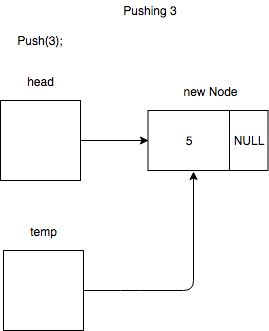
\includegraphics[scale=0.5]{push(5).jpg}
    \caption{Setting temp node}
  \end{figure}
  It now creates a new node and sets head to the newly created node.
  \begin{figure}[H]
    \centering
    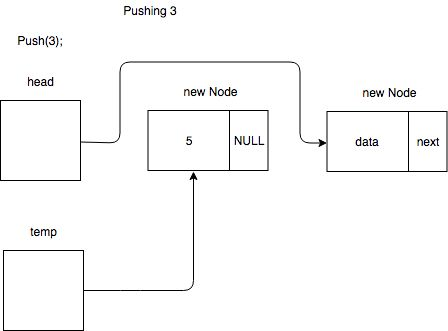
\includegraphics[scale=0.5]{push(6).jpeg}
    \caption{Setting head to the new node}
  \end{figure}
  It sets the newly created node's next pointer to the node being pointed by temp.
  \begin{figure}[H]
    \centering
    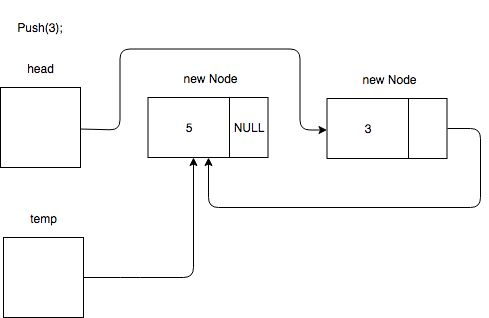
\includegraphics[scale=0.5]{push(7).jpg}
    \caption{Setting next pointer}
  \end{figure}
  The temp gets destroyed since it was a local variable of the function and 3 is added succesfully.
  \textsc{\begin{figure}[H]
      \centering
      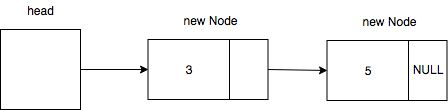
\includegraphics[scale=0.5]{push(8).jpeg}
      \caption{Succesful Push(3) operation}
    \end{figure}}
\end{example}
\newpage
\paragraph{Implementing Pop() Operation}
Inside the class of Stack, we will declare and define a function "Pop()" in public.
\begin{lstlisting}
  int Pop()
  {
    int val = -1;
    if(head != NULL)
    {
      Node* temp = head;
      head = head->next;
      val = temp->data;
      delete temp;
      temp = NULL;
    }
    return val;
  }
\end{lstlisting}
Let's visualize an example of Pop() operation
\begin{example}
  \begin{lstlisting}
    
    stack.Pop();
  \end{lstlisting}
  This is the stack on which pop() will be called.
  \begin{figure}[H]
    \centering
    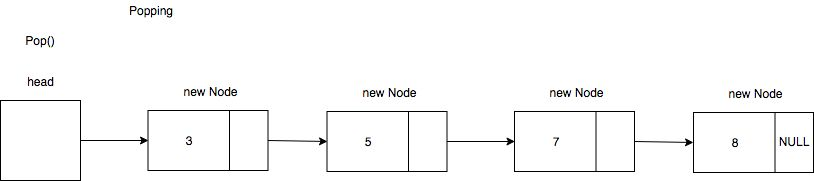
\includegraphics[scale=0.5]{pop(1).jpeg}
    \caption{Stack before pop()}
  \end{figure} ~\\
  After checking the head pointer if it is not NULL, it creates a temp pointer and stores the address of node pointed by head in it.
  \begin{figure}[H]
    \centering
    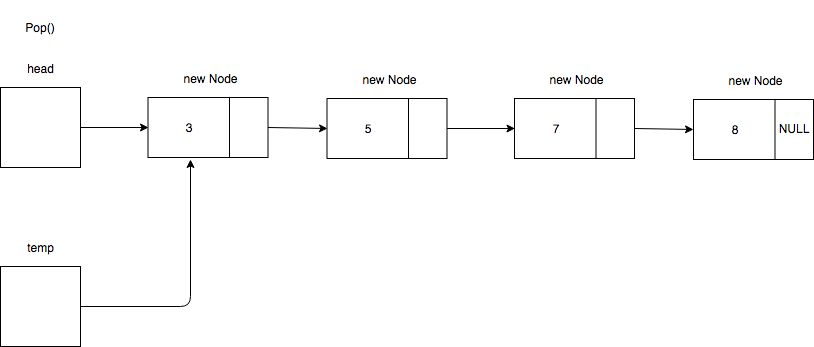
\includegraphics[scale=0.5]{pop(2).jpeg}
    \caption{Creating temp pointer}
  \end{figure} ~\\
  It updates the head pointer to the node next to head
  \begin{figure}[H]
    \centering
    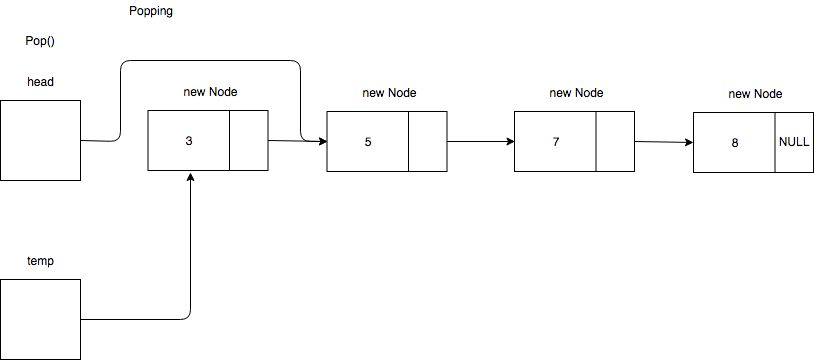
\includegraphics[scale=0.5]{pop(3).jpeg}
    \caption{Updating head pointer}
  \end{figure} ~\\
  It now deletes the node pointed by temp.
  \begin{figure}[H]
    \centering
    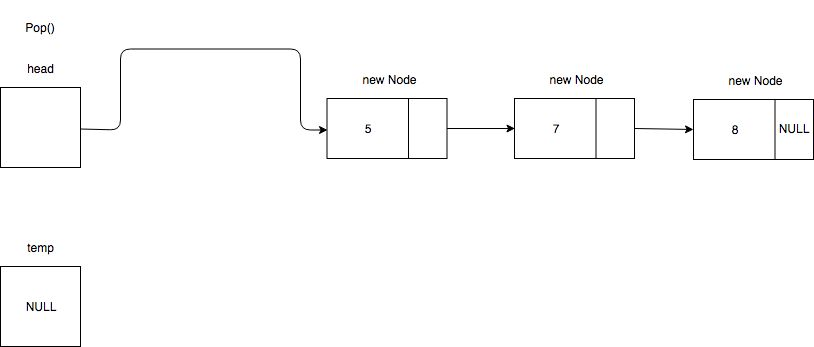
\includegraphics[scale=0.5]{pop(4).jpeg}
    \caption{Deleting the node pointed by temp}
  \end{figure} ~\\
  The temp pointer then gets destroyed and stack is updated successfully.
  \begin{figure}[H]
    \centering
    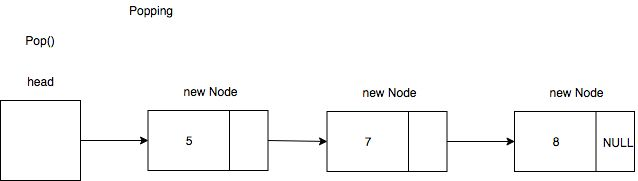
\includegraphics[scale=0.5]{pop(5).jpeg}
    \caption{Succesful pop() operation}
  \end{figure}
\end{example} ~\\
\paragraph{Implementing Show() function}
The Show()  function allows to output all the values in the stack. \\
Inside the class of Stack, we will declare and define a function "void Show()" in public.
\begin{lstlisting}
  void Show()
  Node* temp = head;
  while(temp!=NULL)
  {
    std::cout<<temp->data<<std::endl;
    temp = temp->next;
  }
\end{lstlisting}

Let's visualize an example of Show() operation
\begin{example}
  \begin{lstlisting}
    
    stack.Show();
  \end{lstlisting}
  Creating the temp pointer and points it to the node pointed by head.
  \begin{figure}[H]
    \centering
    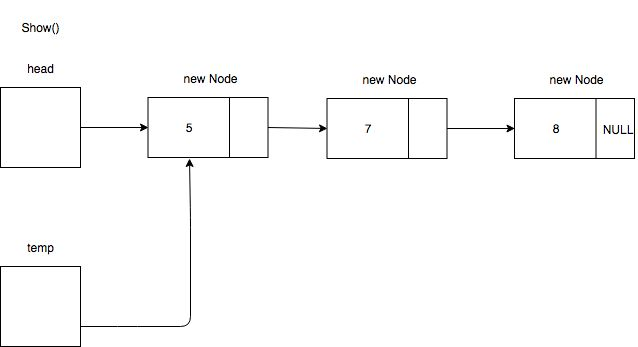
\includegraphics[scale=0.5]{show(1).jpeg}
    \caption{Creating temp pointer}
  \end{figure} ~\\
  Now it outputs the vaue stored in the node pointed by temp.
  \begin{figure}[H]
    \centering
    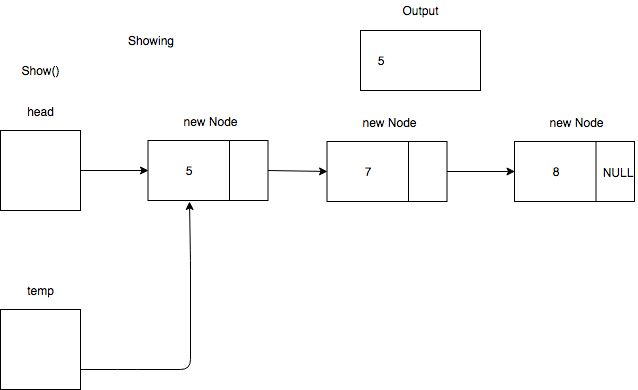
\includegraphics[scale=0.5]{show(2).jpeg}
    \caption{Outputting first value}
  \end{figure} ~\\
  It updates the temp pointer and moves to the next node. Then it outputs the value of the node pointed by temp.
  \begin{figure}[H]
    \centering
    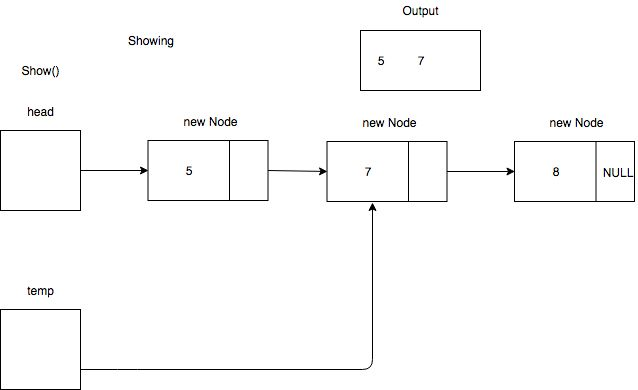
\includegraphics[scale=0.5]{show(3).jpeg}
    \caption{Updating temp pointer and outputting value}
  \end{figure} ~\\
  It repeats the updating of temp pointer and outputs the value
  \begin{figure}[H]
    \centering
    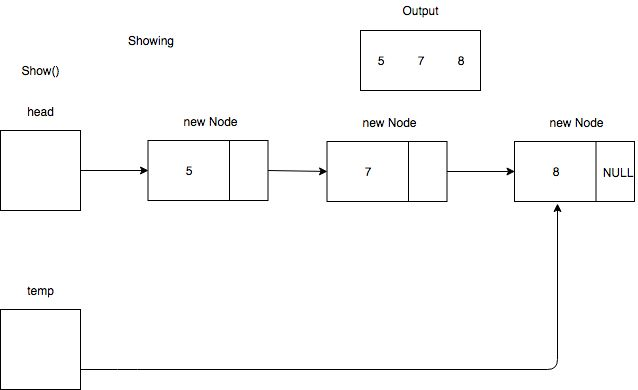
\includegraphics[scale=0.5]{show(4).jpeg}
    \caption{Updating the temp pointer to the third node and outputs the value}
  \end{figure} ~\\
  The loop gets stopped now because the temp is now set to NULL.
  \begin{figure}[H]
    \centering
    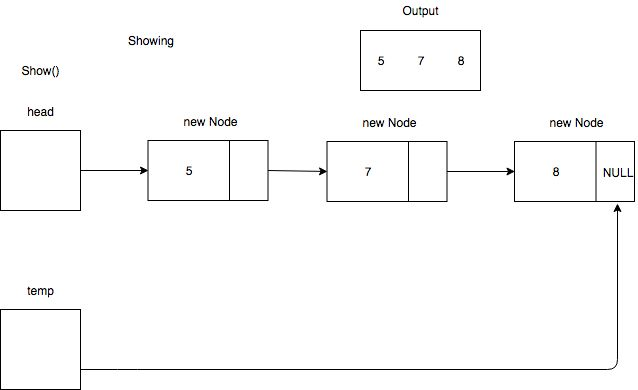
\includegraphics[scale=0.5]{show(5).jpeg}
    \caption{Updating the temp pointer to the third node and outputs the value}
  \end{figure}
\end{example}
\newpage
\section{Problems}\index{Problems}
\begin{problem}
  Implement the isEmpty() function in your Stack class. The function should return true if the stack is empty and return false if not.
  \paragraph{Instructions}
  \begin{itemize}
  \item Think about the value stored in head pointer when the stack is Empty
  \end{itemize}
\end{problem}
~\\
\begin{problem}
  Implement the  functions Top() and Bottom() in your Stack class. The Top() function should return the top element of the stack. The Bottom() function should return the element on the bottom of the stack.
  \paragraph{Instructions}
  \begin{itemize}
  \item Top() function is easy to implement after doing the problem above. Use head pointer to implement this function
  \item For Bottom() function, think how to iterate over the stack till the bottom using only head pointer and a temporary pointer.
  \end{itemize}
\end{problem}

\newpage
\section{Solution}
\begin{lstlisting}[language=C++]
  // ... copy and paste your code
\end{lstlisting}

\newpage
\section{Student Feedback}
\textbf{What did you learn from this lab?}\\
\noindent\fbox{\parbox{\textwidth}{
    % Your feedback here.
  }
}\\
\textbf{What part of the lab is still unclear to you?}\\
\noindent\fbox{\parbox{\textwidth}{
    % Your feedback here.
  }
}\\
\textbf{What can be improved in this lab?}\\ 
\noindent\fbox{\parbox{\textwidth}{
    % Your feedback here.
  }
}


\newpage
%----------------------------------------------------------------------------------------

\chapterimage{chapter_head_2.pdf} % Chapter heading image
\chapter{Constructors in C++ \hspace{36mm} {\textsc{\small SCRIPTED BY : MINHAJ AHMED, ABDUL RAFAY AND TAJ M KHAN}}}

\section{Objective}\index{Objective}

You know about C++'s user-defined types (struct and class) and about their members i.e. member variables and member functions. In this lab, you will learn

\begin{itemize}
	\item The different types of Constructors.
	\item Overloaded Constructors.
	\item Copy Constructors.
	\item Destructors
	\item Array of Pointers.
\end{itemize}

%------------------------------------------------

\section{Key Concepts}\index{Key Concepts}

\subsection{Constructors}

Constructors are special member functions of a class that are used for initializing Objects of that class. They are defined within the class and have the same name as the class. They are automatically called upon the creation of an object. Their return type is not specified in the code. If we don't specify a constructor, C++ generates a default constructor that doesn't take any parameters and has an empty body. Suppose you have got a structure Date and you declare a variable of type Date in main():

%code
\begin{lstlisting}[language=C++, caption = Uninitialized members]
struct Date 
{
	int d,m,y;
};

int main() 
{
	Date today;
	return 0;
}
\end{lstlisting}

\noindent What are the values for member variables d, m, and y in today? Take a guess and then verify it by outputting the values on the screen. Now, you know, about variables, that you've got to initialize them. Therefore, the above code would have garbage values for the members of today. One solution could be to give them values before using them:
% [TODO] confirm the garbage value claim, as class members might be default initialized!
%code
\begin{lstlisting}[language=C++, caption = Initializing members]
struct Date 
{
	int d,m,y;
};

int main()
{
	Date today; 
	today.d=7;today.m=12;today.y=2018;
	return 0;
}
\end{lstlisting}

\noindent What if you had declared 5 different variables of type Date ? What if you had declared an array of 100 Dates ? Initializing this way would be a pain! (ok, the array thing could be done in a loop but still ...). What if you forgot to initialize your objects ? C++ provides a better mechanism.
\smallskip
~\\

\noindent C++ allows you to define special functions for this purpose of initialization. These functions are called constructors. Since constructors are special functions they have their peculiarities:

\smallskip
%~\\

\noindent Syntax wise:
\begin{itemize}
	%\item [$-$] % use - instead of bullet
	\item [$-$] The name of a constructor is exactly the same as the name of the struct/class it is supposed to initialize.
	\item [$-$] Unlike normal functions, constructors do not have a return type. Not even void!
\end{itemize}

\smallskip
%~\\

\noindent Behaviour wise:
\begin{itemize}
	\item[$-$] Constructors get called automatically, whenever an object of that type is created.
	\item[$-$] While you can do anything in a constructor, their primary purpose is to initialize the type's member variables.
\end{itemize}

\noindent So, using a constructor, now our above code becomes:
%code
\begin{lstlisting}[language=C++, caption = Constructor]
struct Date 
{
	int d,m,y;
	Date()
	{
		d=7;m=12;y=2018;
	}
};

int main() 
{
	Date today;
	return 0;
}
\end{lstlisting}

\noindent The above code is exactly equal to the previous code with some superior qualities. Let's see what's there. Inside the struct Date, we've defined a member function whose name is, surprise, exactly the same as the name of the struct! This is the constructor. See how, inside the constructor, we can access the member variables directly, instead of prefixing each with the name of the variable and the dot operator each time ? Our code has become briefer and cleaner. In the function main(), we declare a variable named today of type Date. What are the values of its member variables at that point ? Remember that bit about constructors being called automatically whenever an object of that type is created ? Well, today is an object of type Date, so, when it's created, Date's constructor will be called for it. The code inside the constructor would be executed and it will assign the values 5, 12, and 2018 to members d, m, and y, respectively of the object today. See how after the declaration of today, it's already initialized. 

Now coming back to that earlier question of suppose you had declared 5 different variables of type Date ? Well, the constructor would've been called for each one of them and would have initialized the member variables of each of those objects. What if you'd declared an array of 100 Date objects ? You start to see the benefits of automatic initialization via constructors. And, you can afford to forget about forgetting to initialize the objects.

\subsection{Constructor Overloading}

Like normal functions, constructors can be overloaded, which means that you can have more than one constructors inside a user defined type. What's the advantage of having multiple constructors ? Well, you might want to initialize your objects differently each time they are created. As an example, let's take our favourite Date structure. Right now, every time you create an object of Date, it gets initialized to 07/12/2018. Suppose you want to create an object that where you want to specify the value for day at the time of initialization but would prefer the month and the year to be initialized to the default values. Clearly, the above code does not provide for this. Another time, you might want to be able to specify the day as well as the month at the time of initialization but not the year. How about being able to specify all three at the time of creation ? Overloaded constructors in C++ help you cover all the cases of initialization by letting you specify a constructor for each occasion:
%code
\begin{lstlisting}[language=C++, caption = Overloaded constructors]
struct Date 
{
	int d,m,y;
	Date(){ d=7;m=12;y=2018; } 
	Date (int day) { d=day;m=12;y=2018; } 
	Date (int day, int month) { d=day;m=month;y=2018; } 
	Date (int day, int month, int year) { d=day;m=month;y=year; } 
};

int main()
{
	Date d0;	//d=7, m=12, y=2018
	Date d1(15);	//d=15, m=12, y=2018
	Date d2(15, 11);	//d=15, m=11, y=2018
	Date d3(15, 11, 2003);	//d=15, m=11, y=2003
	//Date d4(15, 11, 2003, 33);//Error: no matching ctor.
	// ... code that does something
	return 0;
}
\end{lstlisting}

\noindent In main(), when we create an object of type Date, we pass it different values in function-style arguments. Based on the number and types of values passed to each variable (remember, these are variables not functions!), the compiler will select the appropriate constructor it can call to initialize that particular object while passing the values to that constructor. So, in the above code, no value is being given to the object d0 of type Date so the compiler will look for a constructor of type Date which does not take any arguments. Finding that the first constructor matches this situation will call it and which will assign the default values to all three members of d0. For the object d1, we are passing it the value 15, it'll see that there's one constructor in Date which takes on argument of type integer. This constructor will be called for d1 and the value 15 will be passed in the function parameter day of the constructor 2. This constructor will initialize the member d with the value passed in parameter day and put default values in members m and y. Similarly, constructors 3 and 4 will be called to initialize the objects d2 and d3. Thus in providing multiple constructors for a type, we give the user flexibility to initialize objects in multiple manners.

Using default arguments can limit the number of constructors you've to define e.g., the above struct can be defined as under without any loss of functionality:
%code
\begin{lstlisting}[language=C++, caption = Default arguments]
struct Date 
{
	int d,m,y;
	Date (int day=7, int month=12, int year=2018)
	{
		d=day;
		m=month;
		y=year;
	}
};
\end{lstlisting}


%C++ 11 stuff
%Date today = Date {7,12,2018}; // initializer_list
%Date today {7,12,2018};

% introduce destructors. will pick up ctors later.
\section{Destructors}
Just like constructors let you execute code and do stuff (initialize variables) when variables/objects are created, C++ provides you a mechanism to be able to execute code and do stuff when variables/objects are destroyed i.e., you know, when they go out of scope or are deleted. This is done via Destructors which, like constructors, are special functions in a user-defined type with the following differences:

\noindent Syntax wise:
\begin{itemize}
	\item[$-$] a destructor's name is the type's name preceded by the character tilda '\textasciitilde'
	\item[$-$] destructors don't take any arguments
	\item[$-$] therefore, destructors cannot be overloaded.
\end{itemize}

\noindent Behaviour wise:
\begin{itemize}
	\item[$-$] Destructors are called when an object goes out of scope or is otherwise destroyed
	\item[$-$] The primary function, no pun intended, of the destructors is to perform clean up and free up any resources that need freeing.
\end{itemize}
%use the Date type to show that default dtors are usually enough
Suppose you want to built your very own string type:
%code
\begin{lstlisting}[language=C++, caption = struct MyString]
struct MyString 
{
	int size;
	char *str;
	
	MyString()
	{
		size=-1; str=NULL;
	} 
	MyString(int sz)
	{
		size=sz;
		str=new char[size+1];
		if(str==NULL)
		{
			cout<<"Error allocating memory"<<endl;
			//exit(-1);
		} 
		for(int i=0; i<size; i++)
			str[i]='a'+i%26; //repeat a-z
		str[size]='\0'; // terminating NULL
	}
}; // end struct MyString
\end{lstlisting}

The struct maintains an integer to store the size of the string and a character array to store the actual string. [If someone's thinking that you don't actually need the integer to store the size, you are absolutely right but, for pedagogical reasons plz excuse our inefficiency.] We provide two constructors: one for default values and one to create a string of specific size initialized to lower-case alphabet. Now you may use this type in your code:
%code
\begin{lstlisting}[language=C++, caption = Use MyString in main()]
int main() 
{
	// .... your code
	for(int i=0; i<23; i++)
	{
		Mystring s(i);
		cout<<s.str<<endl;
		// ... you do ur stuff
	}
	return 0;
}
\end{lstlisting}

What's going on in the above code, memory wise ? Inside the for loop, your user-defined strings are being created and used. What's the scope, life time, of these objects ? What happens to the memory each one of them allocates for it's corresponding character array ? You know that if you allocate memory dynamically, as it's being done in these constructors, it is your responsibility to free it. Is the memory being freed ? If no, what what can we do ? \smallskip
~\\
\noindent As responsible programmers, we should free this memory. One way could be:
%code
\begin{lstlisting}[language=C++, caption = Free memory in main()]
int main() 
{
	// .... your code
	for(int i=0; i<1000; i++)
	{
		Mystring s(i);
		cout<<s.str<<endl;
		// ... you do ur stuff
		
		delete [] s.str;
	}
	return 0;
}

\end{lstlisting}

\noindent This approach would require you to keep track of the life time of each and every MyString object in your program and free their internal character arrays at appropriate times, a huge hassle. That's where C++ destructors jump to your rescue. The key point is that we will not be needing the memory once the object is destroyed. If only we could have this clean up code automatically executed for each object whenever it is destroyed, we needn't worry about keeping track of their life times! The definition of our type becomes:
%code
\begin{lstlisting}[language=C++, caption = Destructor]
struct MyString 
{
	int size;
	char *str;
	MyString()
	{
		size=-1; str=NULL;
	} 
	MyString(int sz)
	{
		size=sz;
		str=new char[size+1];
		if(str==NULL)
		{
			cout<<"Error memory"<<endl;
			exit(-1);
		} 
	for(int i=0; i<size; i++)
		str[i]='a'+i%26;
	str[size]='\0';
	}
	
	// dtor
	~MyString()
	{
		if (str!=NULL)
		{
			delete [] str;
			str=NULL;
		} 
		size=-1; 
	}

}; // end struct MyString
\end{lstlisting}

And we needn't worry about freeing the memory for MyString in our code any more.

\section{Copy Constructor}
Often in our code, we need to create new objects and initialize them to the contents of existing objects i.e. we need the new objects to be copies of the existing objects. Consider the following code:
%code
\begin{lstlisting}[language=C++, caption = Need for Copy Ctor]
int main() 
{
	int y = 5;
	Date d (07,12,2018);
	MyString s (28);
	
	cout<<"initial values:"<<endl;
	cout<<"y = "<<y<<endl;
	cout<<"d = "<<d.d<<"/"<<d.m<<"/"<<d.y<<endl;
	cout<<"s = "<<s.str<<endl;
	
	for(int i=0; i<10; i++)
	{	
		int yy = y;
		Date dd = d;
		MyString ss = s;
		
		// ... you code here
	}
	
	cout<<"final values:"<<endl;
	cout<<"y = "<<y<<endl;
	cout<<"d = "<<d.d<<"/"<<d.m<<"/"<<d.y<<endl;
	cout<<"s = "<<s.str<<endl;
	
	cout<<"hooray!!!"<<endl;
	return 0;
}
\end{lstlisting}

\noindent Observe the output when you run it. What happens ?
\smallskip
~\\

\noindent By default when we copy objects, a byte-wise copy is done for each member i.e. for each member of the existing object, the value of that member is copied in its counter part in the newly created object. That worked perfectly well for all except one of the types in our program. Can you dig out the reason ?

Inside the for loop, when the object ss is initialized from the object s, a default member-wise copy is done. Which results in assigning the value of the character pointer s.str to its counterpart ss.str. They both are now pointing to the same memory location. So far, so good. At the end of the for loop, the scope of ss ends and, since it's going to be destroyed, its destructor is called which frees up the character array being pointed to by ss.str pointer (remember, s.str is still pointing to the same memory). In the next iteration, the object ss is created again and ss.str is initialized to s.str (pointing to the memory location which's been freed). When it goes out of scope, the destructor tries to free the ss.str which is pointing to a memory location which's already been freed. You can't free a memory which's not allocated any more, hence the problem. What to do ?

Again, C++ has figured it out for you. It provides a special constructor, called copy constructor, which is called when the object of a type is created from an existing object. The existing object is passed as an argument to this copy constructor and we can write code to construct the new object to our satisfaction if we do not like the default copying operation. We can add a copy constructor to our code:
%code
\begin{lstlisting}[language=C++, caption = Copy Constructor]
struct MyString 
{
	int size;
	char *str;
	
	MyString(){size=-1; str=NULL;} 
	MyString(int sz)
	{
		size=sz;
		str=new char[size+1];
		if(str==NULL)
		{
			cout<<"Error memory"<<endl;
			exit(-1);
		} 
		for(int i=0; i<size; i++)
			str[i]='a'+i%26;
		str[size]='\0';
	}
	
	// copy constructor
	MyString(MyString& const rhs)
	{
		size=rhs.size;
		str=new char[size+1];
		if(str==NULL)
		{
			cout<<"Error allocating memory"<<endl;
			//exit(-1);
		} 
		for(int i=0; i<size; i++)
			str[i]=rhs.str[i];
		str[size]='\0';
	}	
	
	// dtor
	~MyString()
	{
		if (str!=NULL)
		{
			delete [] str;
			str=NULL;
		} 
		size=-1; 
	}
	

}; // end struct MyString
\end{lstlisting}

\noindent This copy constructor will be called whenever an object of MyString would be created from an existing object with the existing object being passed as a parameter in the reference variable rhs. See how instead of copying the address of the existing object in the pointer str, we allocate separate memory for the string of the new object being constructed and copy the elements of the string of the existing object to this newly allocated array one by one. After construction, both the existing and the newly formed object have their separated allocated memories containing the separate copies of the strings. Thus when the local object, i.e ss,  will go out of scope, its destructor will free up it's own allocated memory, leaving the memory for the string of the original existing object, i.e. s, intact.


\section{Defaults}
If you do not declare a constructor or destructor in an object, the C++ standard specifies that your compile will generate for you:
\begin{itemize}
	\item[$-$] a default constructor which would:
	\begin{itemize}
		\item leave the built-in types (int, float, pointers, etc.) to an uninitialized value
		\item call the default constructor on class members
	\end{itemize}
	\item[$-$] a default copy constructor which would do a member wise copy of the existing object to the members of the new object
	\item[$-$] a default destructor which would do nothing
	%\item[]$-$] a default move constructor
\end{itemize}

% From C++ onwards, there are move constructors as well.


\newpage
\section{Problems}\index{Problems}

\begin{problem} Create a class point\_3D which should store the three dimensional coordinates of a point as x, y, and z. The following code in main should behave as in commments:
	%code
	\begin{lstlisting}[language=C++, caption = Create class point\_3D]
	int main()
	{
		point_3D p0;	//should initialize x,y,z to 0,0,0
		point_3D p1(23);//should initialize x,y,z to 23,0,0
		point_3D p2(23,33);//should initialize x,y,z to 23,33,0
		point_3D p3(2,3,5);//should initialize x,y,z to 2,3,5
		
		p3.display();	//outputs pt on screen as (2,3,5)
		
		point_3D p4 = p2; //should initialize xyz in p4 to 23,33,0
		
		//dynamically create some points and display them.
		int x=0;
		cout<<"enter the number of pts u want to create:"<<endl;
		cin>>x;
		point_3D *p = new point_3D[x];
		for(int i=0; i<x; i++)
			(p+i)->display();
		delete [] p;		
		return 0;
	}
	\end{lstlisting}
	
\noindent Based on your understanding, guess whether you need to make any constructor(s), destructor.\\
\end{problem}
\begin{problem} Create a class polygon\_2D which stores the vertices of a polygon as a set of point\_3D objects with the z-coordinate always initialized to 0. When creating an object of polygon\_2D, the user should be able to specify the number of points in the polygon. i.e.:
	%code
	\begin{lstlisting}[language=C++, caption = Create class polygon\_2D]
	int main() 
	{
		polygon_2D pg; // creates a polygon with zero points
		polygon_2D pg1(3); // creates a polygon with 3 pts i.e a triangle
		polygon_2D pg2(5); // 5 pts i.e a pentagon
		
		pg2.display(); 	// displays the points comprising this polygon. 
		polygon_2D pg3 = pg2;
		pg3.display();
		for(int i=0;i<10;i++)
		{
			polygon_2D pg4 = pg3;
			pg4.display();
		}		
		return 0;
	}
	\end{lstlisting}	
	Based on your understanding, guess whether you need to make any constructor(s), destructor.\\
\end{problem}


\newpage
\section{Solution}
\begin{lstlisting}[language=C++]
  // ... copy and paste your code
\end{lstlisting}

\newpage
\section{Student Feedback}
\textbf{What did you learn from this lab?}\\
\noindent\fbox{\parbox{\textwidth}{
    % Your feedback here.
  }
}\\
\textbf{What part of the lab is still unclear to you?}\\
\noindent\fbox{\parbox{\textwidth}{
    % Your feedback here.
  }
}\\
\textbf{What can be improved in this lab?}\\ 
\noindent\fbox{\parbox{\textwidth}{
    % Your feedback here.
  }
}

\newpage
% ----------------------------------------------------------------------------------------

\chapterimage{chapter_head_2.pdf} % Chapter heading image

\chapter{Inheritance and Abstract Classes \hspace{65mm} {\textsc{\small SCRIPTED BY : NABIHA SHAHID and HAMZA MASROOR}}}

\section{What Is Inheritance?}\index{What Is Inheritance?}

Inheritance enables new classes to inherit the properties and methods of existing classes. We know that an object is a self-contained component that contains properties and methods needed to make a certain type of data useful.Since a class is a blueprint to build a specific type of object and that every object is built from a class, inheritance is a way to express a relationship between these classes.\\
For instance, you want to build a new object that is similar to one that already exists, and instead of creating the new class from scratch, you want to reference the existing class and simply indicate what's different.\\
Using inheritance you can organize your objects into a hierarchy, this often creates easier to understand code, but most importantly it allows you to reuse and organize code more effectively.

\section{Base and Derived Classes}\index{Base and Derived Classes}

A base class is a class, in an object-oriented programming language, from which other classes are derived.A base class may also be called parent class or superclass. Whereas, a derived class is the class through which any defined class type may be inherited.\\
The hierarchical relationship between derived class and base class is known as an “is a” relationship.
\begin{figure}[h]
  \centering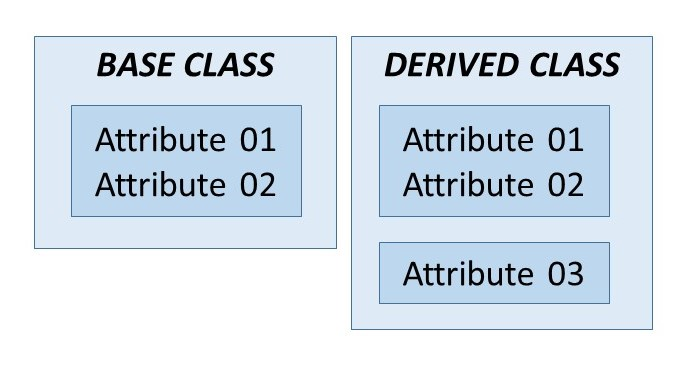
\includegraphics[scale=0.5]{bAse.jpg}
  \caption{Base and Derived Classes}
\end{figure}

\newpage
\section{Example}\index{Example}

For instance, consider a class Animal as the base class through which three derived classes are inherited i.e Lion, Bear and Rabbit.

\begin{figure}[h]
  \centering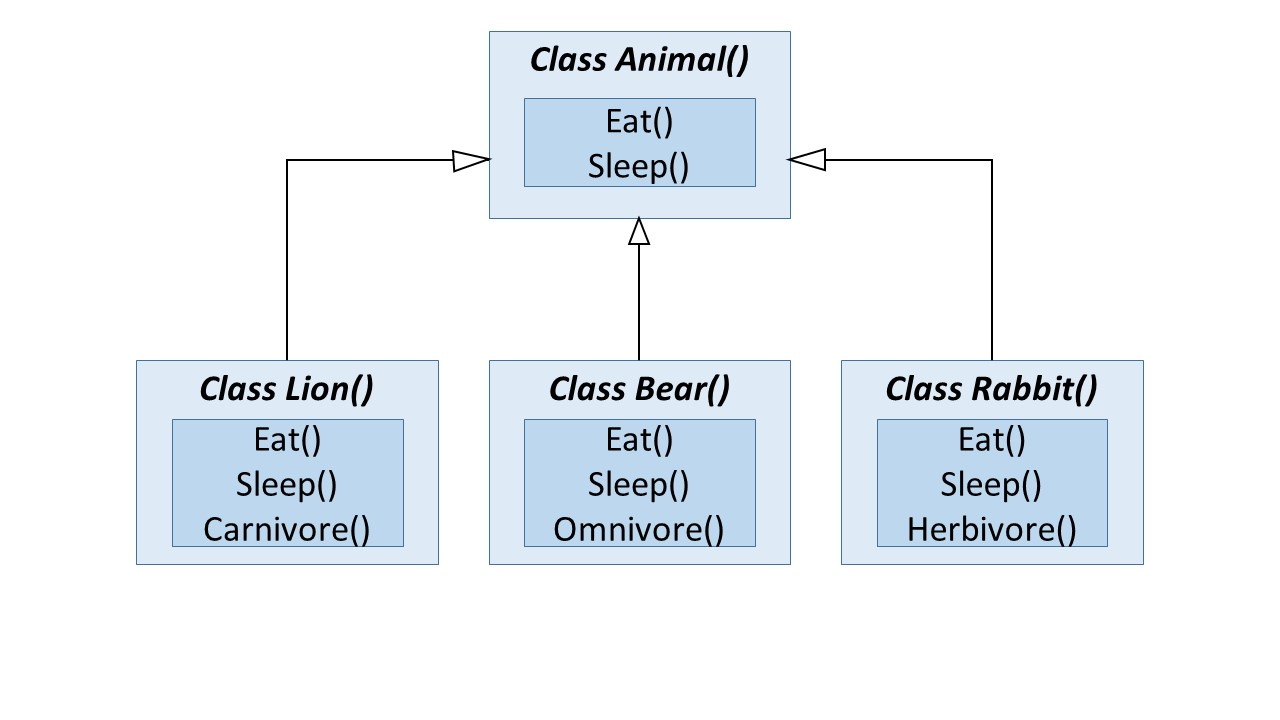
\includegraphics[scale=0.5]{eg.jpg}
  \caption{Example}
\end{figure}
\hfill

\newpage
\section{Implementation}\index{Implementation}
\begin{lstlisting}
  class Animal 
  {
    ... .. ...
  };

  class Lion : public Animal
  {
    ... .. ...
  };

  class Bear : public Animal
  {
    .... .. ...
  };

  class Rabbit : public Animal 
  {
    ... .. ...
  };
\end{lstlisting}
\hfill 
\section{Access Control and Specifiers}
\index{Access Control and Specifiers}
All the non-private members of a base class are accessible by the derived class except for;

\begin{itemize}
\item Constructors, Destructors and Copy Constructors of base.
\item Overloaded Operators of base.
\item Friend Functions of base.
\end{itemize}
Therefore those functions that need not be approachable should be declared private.

\begin{center}
  \begin{tabular}{ |c|c|c|c|c| } 
    \hline
    Access & Public & Protected & Private \\
    \hline
    Same Class & Yes & Yes & Yes \\ 
    Derived Class & Yes & Yes & No \\ 
    Outside Class & Yes & No & No \\ 
    \hline
  \end{tabular}
\end{center}
\begin{lstlisting}
  class base 
  {
    public:
    int atr1;
    protected:
    int atr2;
    private:
    int atr3;
  };

  class publicDerived: public base
  {
    // atr1 is public
    // atr2 is protected
    // atr3 is not accessible as it is a private member
  };

  class protectedDerived: protected base
  {
    // atr1 is protected
    // atr2 is protected
    // atr3 is not accessible as it is a private member
  };

  class privateDerived: private base
  {
    // atr1 is private
    // atr2 is private
    // atr3 is not accessible as it is a private member 
  }
\end{lstlisting}

\section{Type Of Inheritance}
\index{Lists!Types Of Inheritance}
\begin{itemize}
\item \textbf{Public Inheritance} \\
  When deriving a class from a public base class, public members of the base class become public members of the derived class and protected members of the base class become protected members of the derived class. A base class's private members are never accessible directly from a derived class, but can be accessed through calls to the public and protected members of the base class.\\
\item \textbf{Protected Inheritance} \\
  When deriving from a protected base class, public and protected members of the base class become protected members of the derived class.\\
\item \textbf{Private Inheritance} \\
  When deriving from a private base class, public and protected members of the base class become private members of the derived class. 
\end{itemize}

\section{Abstract Classes}
\begin{figure}[h]
  \centering
  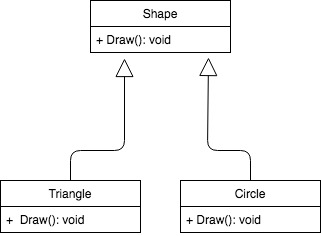
\includegraphics[scale=0.5]{UML.jpeg}
  \caption{UML representation of abstract class}
\end{figure} ~\\
Sometimes implementation of all function cannot be provided in a base class because we don’t know the implementation. Such a class is called \textbf{abstract class}. For example, let Shape be a base class. We cannot provide implementation of function draw() in Shape, but we know every derived class must have implementation of draw(). Similarly an Animal class doesn’t have implementation of move() (assuming that all animals move), but all animals must know how to move. We cannot create objects of abstract classes. For this, we need to have at least one pure virtual function in the class. \\
A \textbf{pure virtual function} (or abstract function) in C++ is a virtual function for which we don’t have implementation, we only declare it. A pure virtual function is declared by assigning 0 in declaration. It's done by the syntax showed below.
\begin{lstlisting}
  // An abstract class
  class Test
  {   
    // Data members of class
    public:
    // Pure Virtual Function
    virtual void show() = 0;

    /* Other members */
  };
\end{lstlisting} ~\\
Let's see an example in whch a pure virtual function is declared in the abstract class and then defined in the derived class.
\begin{example}
  \begin{lstlisting}
    class Base
    {
      int x;
      public:
      virtual void func() = 0;
      int getX() 
      {
        return x; 
      }
    };

    // This class inherits from Base and implements func()
    class Derived: public Base
    {
      int y;
      public:
      void func()
      {
        cout << "func() called";
      }
    };

    int main()
    {
      Derived d;
      d.func();
      return 0;
    }
  \end{lstlisting}
  Now the abstract class has the attribute 'int x' and the function 'int GetX()'. This function will also be the part of derived class and is already defined in the base class. Now the function 'func()' is a pure virtual function which is defined in the base class and is implemented in the derived class. Now, if we create an instance of Derived class, we can access the functions 'GetX()' and 'func()'. The 'GetX()' will be called through the base class and 'func()' will be called through the derived class.
  The program above will output:
  \begin{figure}[h]
    \centering
    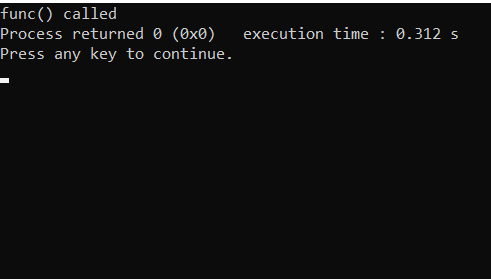
\includegraphics[scale=0.5]{Class.png}
    \caption{Output of implemented pure virtual function}
  \end{figure}
\end{example}
The derived class can also become an abstract class if the pure virtual function declared in base class is not defined in the derived class.
\begin{example}
  \begin{lstlisting}
    class Base
    {
      public:
      virtual void show() = 0;
    };

    class Derived : public Base { };

    int main(void)
    {
      Derived d;
      return 0;
    }
  \end{lstlisting}
\end{example}
\begin{corollary}[Interface vs Abstract classes]
  An interface does not have implementation of any of its methods, it can be considered as a collection of method declarations. In C++, an interface can be simulated by making all methods as pure virtual. In Java, there is a separate keyword for interface.
\end{corollary}

\newpage
\section{Problems} \index{Problems}
\begin{problem}
  Your code should represent a program that defines a class $shape$ carrying a constructor mentioning the width and height. After that define two sub-classes $triangle$ and $rectangle$ , inherit them from the base class shape and calculate the area of the shape $area()$.In the main, define two variables a triangle and a rectangle and then call the $area()$ function in these two varibles.\\
\end{problem}
\begin{problem}
  Write a program with a base class and an inherited class.Both of them should have a method void $display()$ that prints a separate message for both. In the main define a variable for the inherited class and call the $display()$ method on it.\\
\end{problem}
\begin{problem}
  Write a probram with a base class $animal$. Inside it define a name and an age variables, and $setvalue()$ function. Then create two bases variables Dog and Dolphin which write a message telling the age, the name and giving some extra information like color or breed.
\end{problem}
\begin{problem}
  Make an abstract class of Shape with pure virtual function to calculate area. It should also have the attributes for the position of the Shape. The derived classes should be Square, Circle, Trapezium and Rectangle. All derived classes should implement the pure virtual function defined in the base class. 
  \paragraph{Instructions}
  \begin{itemize}
  \item Make a struct for Position to have x and y coordinates.
  \item Define the attributes for dimensions according to the shape in derived classes
  \end{itemize}
\end{problem} ~\\
\begin{problem}
  Make a base class with a pure virtual function. Derive a class from it and declare another pure virtual function in the derived class. Then derive an other class from the first derived class and declare a pure virtual function in it too. And then lastly derive another class from the second derived class, and define all the pure virtual functions in it
\end{problem}

\newpage
\section{Solution}
\begin{lstlisting}[language=C++]
  // ... copy and paste your code
\end{lstlisting}

\newpage
\section{Student Feedback}
\textbf{What did you learn from this lab?}\\
\noindent\fbox{\parbox{\textwidth}{
    % Your feedback here.
  }
}\\
\textbf{What part of the lab is still unclear to you?}\\
\noindent\fbox{\parbox{\textwidth}{
    % Your feedback here.
  }
}\\
\textbf{What can be improved in this lab?}\\ 
\noindent\fbox{\parbox{\textwidth}{
    % Your feedback here.
  }
}

\newpage
\chapterimage{chapter_head_2.pdf} % Chapter heading image
\chapter{Brainstorming and Design \hspace{40mm} {\textsc{\small SCRIPTED BY : UMAIR AZFAR}}}

\section{Making Project Groups}
By this time, you should have made project groups. Your group should have 3 to 4 members so that the amount of work can be distributed evenly among your group members. Choose your group members wisely as they are the key in completing your project.
In this lab, you should sit with your project group members as you will be working with each other in performing various tasks. You will work together in coming up with a project idea after your brain storming session.

\section{Brain Storming}
You will take 15 minutes in coming up with your own original game/application idea that you will work on as your final project for this course. You should take your pen and paper out and write about your project idea individually. The important points that you must follow in coming up with your idea are given as follows:
\begin{itemize}
\item The idea should be about some local context
\item The idea should contain many objects that interact with each other
\item The objects should be inherited from each other
\item If making a game, avoid making games that are top-down shooting games or side scrolling
shooting games.
\item Avoid making games like breakout as they have been done many times before
\end{itemize}
Once your 15 minutes are over, take another 15 minutes to discuss your idea with your teammates and select one idea by the end of the 15 minutes. The next 30 minutes will be spent in coming up with the features of your game/application that you think your project must have. For example, if you are making a game, you need to decide on how the menu screen will look like, what options will the user be able to change. What will the player be doing, what enemies will the player encounter, what objects will be there for interaction, what level will be there and how they will change, etc. For the next 30 minutes, all the groups will present their idea in 5 minutes to the entire class and will receive feedback. They will note down the feedback to further enhance their idea and arrive at a set of features that they think they should be adding to their project.

\section{Design}

This is where your UML 2.0 skills will come in handy. The time you are left with will be spent in you coming up with a good design for your project. You will need to decide the number of objects that your application will have and what will be the relationships between the many classes that you will define. You also need to think about the attributes and the functions that the classes will have. This will be a rough start for your Assignment 6 so you need to pay special attention to it. Over the course of coming weeks till you need to submit Assignment 6 you will need to meet your instructor and come up with a worthwhile plan. You will also need to distribute the tasks among your group members and convey that to your instructor. You will initially make your UML diagrams by pen and paper, but later redraw them using {\tt UMLet}.

\newpage
\section{Student Feedback}
\textbf{What did you learn from this lab?}\\
\noindent\fbox{\parbox{\textwidth}{
    % Your feedback here.
  }
}\\
\textbf{What part of the lab is still unclear to you?}\\
\noindent\fbox{\parbox{\textwidth}{
    % Your feedback here.
  }
}\\
\textbf{What can be improved in this lab?}\\ 
\noindent\fbox{\parbox{\textwidth}{
    % Your feedback here.
  }
}

\newpage
\chapterimage{chapter_head_2.pdf} % Chapter heading image
% ----------------------------------------------------------------------------------------

\chapter{Collision Detection \hspace{38mm} {\textsc{\small SCRIPTED BY : ABDUL RAFAY}}}
\section{Objective}\index{Objective}
In this lab we will learn the concept of collision detection. We will also observe the behavior of each class and their relation with other classes and their objects.
\section{Class Relationship Diagram}index{Class Relationship Diagram}
\begin{figure}[h]
  \centering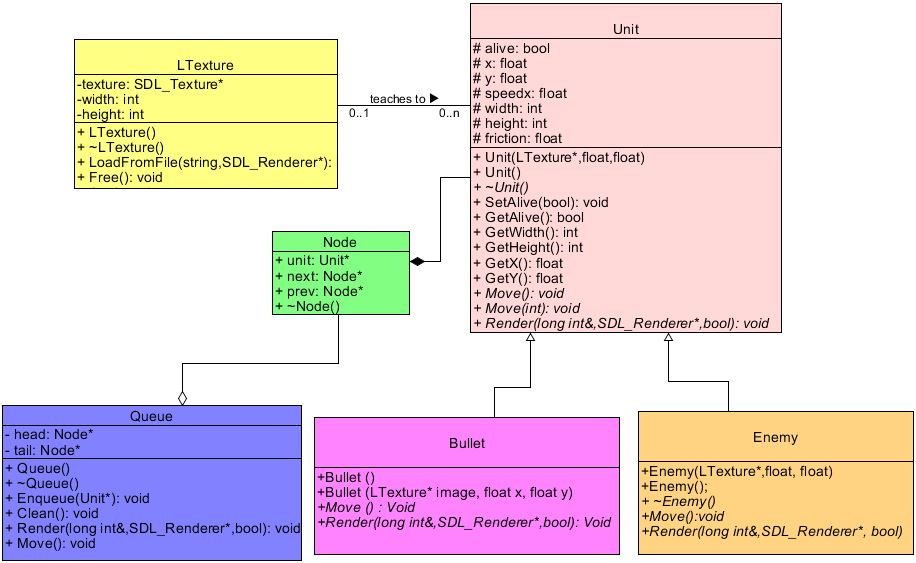
\includegraphics[scale=0.6]{UML.jpg}
  \caption{UML of Task}
\end{figure}
\newpage
\section{Class Wise Description}
\subsection{Unit}
Unit class is the base class for the bullet and enemy class. By default, Unit class's Render() function renders user's plane but since this function is \emph{virtual} it is overridden at the time of rendering enemy or bullet objects. There is also one interesting variable named as friction in this class. This variable is used in the overloaded Move(int) function which smooths out user plane's movement so that it is not too quick or too slow. You should try to change the value of this variable to see the difference in the movement.You are required to use this variable to smoothen the movements of enemy plane when it is trying to dodge the bullet.This class is the building block of the entire game.
\subsection{LTexture}
You are required to go through Lazyfoo tutorials to understand this class.
In its Render() function, parameters of x coordinate and y coordinate are usually reduced by half of the width and height of the plane:\\

x - width/2 , y - height/2\\
\hfill \break
This is done because SDL starts rendering from the top left point of the object but we want this point to be at the center of the rendering object as illustrated in Figure 2.

\begin{figure}[h]
  \centering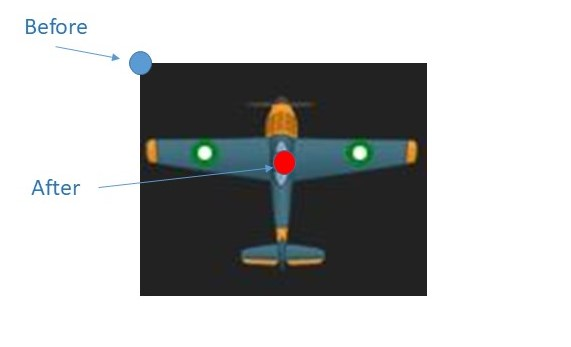
\includegraphics[scale=0.5]{plane.jpg}
  \caption{Rendering coordinates}
\end{figure}

\subsection{Queue and Node}
Queue class is your storage container which keeps tack of all the objects that are currently active. Once the enemy plane or bullet passes the screen size it should be removed from this container and deallocated. Similarly , if an enemy plane is destroyed it must also be removed from this container. This container is essential to determine which enemy plane among all the active enemies is to be destroyed in case it is hit or to determine which enemy plane will be trying to dodge the bullet. 

\subsection{Bullet}
Bullet class is similar to the enemies class as it is also inherited from the Units class. However, x coordinate of bullet object is crucial to determine which plane is expected to be hit by the bullet and consequently which side (right or left) will the enemy plane be moving in order to dodge this bullet.Y coordinate of the bullet should determine at what point of time should the enemy plane make any movements.To make the game more interesting, this distance from bullet to enemy plane should be random so that there is equal chance of plane getting hit and plane dodging the bullet.

\section{Problems}\index{Problems}
Edit the code that has been provided to you to add following functionality to the game:\\
\begin{problem} There should be an explosion whenever bullet hits the enemy plane.\\
\end{problem}
\begin{problem} Enemy plane should detect the bullet and it must try to dodge it.\\
\end{problem}
\begin{problem} If the enemy is hit, it should be destroyed and removed from the game.
\end{problem}

\begin{tcolorbox}[width=\textwidth,colback={white},title={KEYNOTE},colbacktitle=purple!50!white,coltitle=black] 
  Please go through Lesson 27 of Lazyfoo regarding collision detection.
\end{tcolorbox}

\newpage
\section{Solution}
\begin{lstlisting}[language=C++]
  // ... copy and paste your code
\end{lstlisting}

\newpage
\section{Student Feedback}\index{Student Feedback}
\textbf{What did you learn from this lab?}\\
\noindent\fbox{\parbox{\textwidth}{
    % Your feedback here.
  }
}\\
\textbf{What part of the lab is still unclear to you?}\\
\noindent\fbox{\parbox{\textwidth}{
    % Your feedback here.
  }
}\\
\textbf{What can be improved in this lab?}\\ 
\noindent\fbox{\parbox{\textwidth}{
    % Your feedback here.
  }
}

\newpage
\chapterimage{chapter_head_2.pdf} % Chapter heading image
% ----------------------------------------------------------------------------------------
\chapter{Templates \hspace{65mm} {\textsc{\small SCRIPTED BY : NABIHA SHAHID}}}

\section{What Are Templates?}\index{What Are Templates?}

Templates are one of the most important tools of C++ which lets you write your code independent of any particular data type. This is done by just passing the data type as a parameter so that we do not have to write the same code for different data types.

\subsection{Example}\index{Example}
A developer might want to use a function for different datatypes, instead of maintaining several code we could just create one function and pass data type as a parameter.\\
There is a single definition of each standard library container, such as vector, but we can define many different kinds of vectors for example, vector <int> or vector <string>.\\
Note that once a vector is initialized with a certain data type it would not work for any other.

\section{Types Of Templates}\index{Types Of Templates}

The concept of templates is used in two different ways.\\
\begin{itemize}
\item Function Templates 
\item Class Templates
\end{itemize}

\section{Function Templates}\index{Function Templates}

As we know that normally functions can only work with a certain set of data types, what makes function templates special is its ability to work with different data types at once.This makes the code manageable too.
\newpage
\subsection{Declaration}\index{Declaration}
\begin{lstlisting}[language=C++, caption= Declaration Of Function Templates]
  template <class Type>
  Type Function(Type arg)
  {
    //function body
  }
\end{lstlisting}

Here, \textbf{\textit{'class'}} is a keyword which could be replaced by 'typename' {(\it{according to the 2017 version})} and \textbf{\textit{'type'}} is a template argument which accepts different datatypes. When we pass an argument of a data type to Function( ), the compiler will generate a new version of Function() for the given data type.\\

\subsection{Example}\index{Example}

\begin{lstlisting}[language=C++, caption= Eg:Function Template to output the greater number
  ]
  #include <iostream>
  
  template <typename Type>
  Type max(Type x, Type y)
  {
    return (x > y) ? x : y;
  }
  
  int main()
  {
    int i = max(3, 7);
    cout << i << '\n';
    
    double d = max(6.34, 18.523);
    cout << d << '\n';
    
    char ch = max('a', '6');
    cout << ch << '\n';
    
    return 0;
  }
\end{lstlisting}
\textbf{Output}
\begin{lstlisting}
  7
  18.523
  a
\end{lstlisting}

\section{Class Templates}\index{Class Templates}
Class functions may also be created just like function templates when perform generic class operations.Instead of expanding your own code by using the same class code wherever it is needed with different data types, you just simply create a class template!

\subsection{Declaration}\index{Declaration}
\begin{lstlisting}[language=C++, caption= Declaration Of Class Templates]
  template <class Type>
  class className
  {
    ...
    public:
    Type var;
    Type Function(Type arg);
    ... 
  };
\end{lstlisting}

\section{Some Important Facts}\index{Some ImportanT Facts}

Ever wondered if we could pass more than one data type as argument to templates? Then Yes, have a look at this.

\begin{lstlisting}[language=C++, caption= Important Fact 1]
  #include<iostream>
  using namespace std;
  
  template<class T1, class T2>
  class Imp {
    T1 x;
    T2 y;
    Public:
    Imp() {cout<<"Constructor Called"<<endl;}
  };
  
  int main()  
  {
    Imp<char, char> a;
    Imp<int, double> b;
    return 0;
  }
\end{lstlisting}

Or if we could specify default arguments to templates? Yes, have a look.
\begin{lstlisting}[language=C++, caption= Important Fact 2]
  #include<iostream>
  using namespace std;
  
  template<class T1, class T2 = char>
  class Imp {
    public:
    T1 x;
    T2 y;
    Imp() { cout<<"Constructor Called"<<endl; }
  };
  
  int main()  {
    Imp<char> a; 
    return 0;
  }
\end{lstlisting}

\section{Problems}\index{Problems}

\begin{problem} Generate a program that swaps data values using function templates.\\
\end{problem}
\begin{problem} Generate a simple calculator using class templates which adds, subtracts , multiplies and divides.\\
\end{problem}
\begin{problem} Write a code that defines class Stack <> and implement functions to push and pop elements from stack using templates.\\
\end{problem}
\begin{problem} Create a program demonstrating Quick Sort Algorithm using templates.
\end{problem}

\newpage
\section{Solution}
\begin{lstlisting}[language=C++]
  // ... copy and paste your code
\end{lstlisting}

\newpage
\section{Student Feedback}\index{Student Feedback}
\textbf{What did you learn from this lab?}\\
\noindent\fbox{\parbox{\textwidth}{
    % Your feedback here.
  }
}\\
\textbf{What part of the lab is still unclear to you?}\\
\noindent\fbox{\parbox{\textwidth}{
    % Your feedback here.
  }
}\\
\textbf{What can be improved in this lab?}\\ 
\noindent\fbox{\parbox{\textwidth}{
    % Your feedback here.
  }
}

\newpage
\pagestyle{empty} % No headers

\cleardoublepage % Forces the first chapter to start on an odd page so it's on the right

\pagestyle{fancy} % Print headers again

\chapterimage{chapter_head_2.pdf} % Chapter heading image

% ----------------------------------------------------------------------------------------
\chapter{Rendering Text and Buttons in SDL \hspace{1mm} {\textsc{\small SCRIPTED BY : MINHAJ AHMED}}}

\section{Objective}\index{Objective}

In this lab, you will learn to

\begin{itemize}
\item Render Bitmap text on the SDL Window.
\item Render a button on the SDL Window.
\item Make the button interactive.
\end{itemize}

\section{Key Concepts}\index{Key Concepts}

\subsection{Sprite Sheets}
A Sprite Sheet is an image which contains multiple smaller images. These images could either be static or they might contain animations. Frames for animations can also be added into the sprite sheet. Combining the small images in one big image improves the game performance, reduces the memory usage and speeds up the startup time of the game, since only one image file has to be loaded which can be clipped for use. Example Sprite Sheet shown in Figure 1.1.

\begin{figure}[h]
  \centering
  \fbox{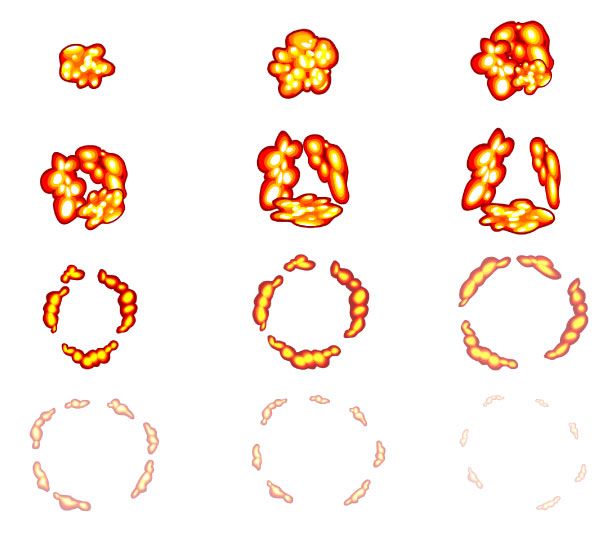
\includegraphics[scale=0.3]{spr.jpg}}
  % 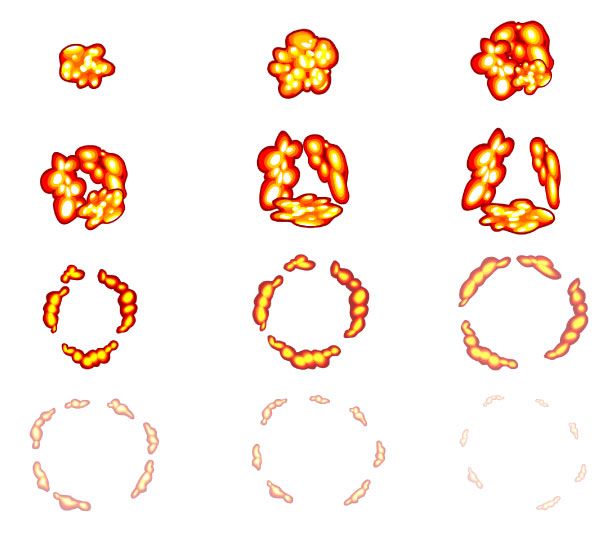
\includegraphics[scale=0.3]{spr.jpg}
  \caption{Sprite Sheet for an explosion}
  % \label{my_label}
\end{figure}


\subsection{Bitmap Fonts}

BitMap Fonts consist of glyphs on a spritesheet, which can be loaded into the program using SDL Library, and characters from it can be rendered on the screen. The rendering of a single glyph requires clipping from the spritesheet, i.e take only some part of the spritesheet and render it on the screen. Example of such a font in a sprite sheet is given below.

\begin{figure}[h]
  \centering
  
\includegraphics[scale=0.3]{font.png}
  \caption{SpriteSheet for a bitmap Font}
  % \label{my_label}
\end{figure}


\subsection{Texture}

Textures are images that are used in 3D games on 3D objects, 2D planes in 3D space, or GUI elements. They may be stored in the RAM or the VRAM. In SDL, a texture is a structure that contains pixel data from images, graphics or sprites. 

\subsection{Rendering Bitmap Text}

For rendering Bitmap Text, we will need to create a \texttt{Character} Class in order to render Characters from a spritesheet. For rendering words or text, we will need an array or list of \texttt{Character} Objects. For this purpose we will have to create another class called \texttt{Text} which will contain the \texttt{Character} Objects and will render them on the screen. In the \texttt{Text} Class, we can choose either a linked list or an array of \texttt{Character} Objects as the data structure. The Text Class will then render each Character on the screen thus, rendering the whole Bitmap Text on the SDL Window.

\section{Syntax Examples}\index{Syntax Examples}

\subsection{Texture Loading}

For loading Textures, we make a new class \texttt{LTexture} that contains member functions for loading and rendering Textures in SDL. This class only contains functions needed for rendering on the screen. Other functions, for example, for changing the Blend Mode, or the Opacity or for Color Modulation can also be made.

% https://stackoverflow.com/questions/21007329/what-is-a-sdl-renderer/21007477#21007477

\begin{lstlisting}[language=C++, caption={Default, Overloaded and Copy Constructors}]
  class LTexture
  {
    public:
    LTexture();                     //Initializes variables
    {
      texture = NULL;
      width = 0;
      height = 0;
    }
    void free()
    {
      if(texture != NULL)
      {
        SDL_DestroyTexture(texture);
        texture = NULL;
        width = 0;
        height = 0;
      }
    }
    ~LTexture();                    //Deallocates memory
    {
      free();
    }
    //Renders texture at given point
    void render(int x, int y, SDL_Renderer* gRenderer,
    SDL_Rect* clip = NULL)
    {
      //Set rendering space and render to screen
      SDL_Rect renderQuad = { x, y, width, height };
      if( clip != NULL )
      {
        renderQuad.w = clip->w;
        renderQuad.h = clip->h;
      }
      //Render to screen
      SDL_RenderCopy(gRenderer, texture, clip, &renderQuad);
    }
    //Gets image dimensions
    int getWidth()
    {
      return this->width;
    }
    int getHeight()
    {
      return this->height;
    }
    private:
    SDL_Texture* texture; //The actual hardware texture
    int width;
    int height;
  };
\end{lstlisting}

\begin{lstlisting}[language=C++, caption={Use of Array of Pointers and Destructors}]
  bool loadFile(string path);     //Loads image
  {
    free();
    SDL_Texture* newTexture = NULL;
    //Load image at specified path
    SDL_Surface* loadedSurface = IMG_Load(path.c_str());
    if (loadedSurface != NULL)
    {
      SDL_SetColorKey(loadedSurface, SDL_TRUE,
      SDL_MapRGB(loadedSurface->format, r, g, b));
      //Create texture from surface pixels
      newTexture = SDL_CreateTextureFromSurface( 
      gRenderer, loadedSurface);
      
      if (newTexture != NULL)
      {
        width = loadedSurface->w;
        height = loadedSurface->h;
      }
      //Get rid of old loaded surface
      SDL_FreeSurface( loadedSurface );
    }
    texture = newTexture;
    return texture != NULL;
  }
\end{lstlisting}

Now, that we have made our \texttt{LTexture} Class, we can now render images on the screen, but we still need our \texttt{Text} ad \texttt{Character} Classes.

\subsection{Rendering Characters on the Screen}

Rendering a character on the screen would require us to specify the position, the texture that contains our font spritesheet and an \texttt{SDL\_Rect} Object telling us the coordinates for clipping the character from the spritesheet.

\begin{lstlisting}[language=C++, caption={Use of Array of Pointers and Destructors}]
  class Character
  {
    public:
    Character();
    Character(char c,LTexture* gSpriteSheetTexture);
    void render(SDL_Renderer* gRenderer);
    void setPosition(int x, int y);
    void setChar(char c);
    void setTexture(LTexture* gSpriteSheetTexture, char c);
    private:
    int x,y;
    SDL_Rect charRect;
    char shownChar;
    LTexture* CharTexture;
  };
\end{lstlisting}

The Implementation for this class is below. Since we are only using Capital Letters, we will use only the ASCII codes for Capital Letters (65 to 91) in order to get the characters from the spritesheet. The width and height of the characters have to be found out from the spritesheet.

\begin{lstlisting}[language=C++, caption={Use of Array of Pointers and Destructors}]
  Character::Character(char c,LTexture* gSpriteSheetTexture)
  {
    this->shownChar = c;
    this->CharTexture = gSpriteSheetTexture;
    this->charRect.w = 88;
    this->charRect.h = 99;
    this->setPosition(10, 10);
    this->setChar(c);
  }
  void Character::setTexture(LTexture* gSpriteSheetTexture, char c)
  {
    this->shownChar = c;
    this->CharTexture = gSpriteSheetTexture;
    this->charRect.w = 88;
    this->charRect.h = 99;
    this->setPosition(10, 10);
    this->setChar(c);
  }
  Character::Character(){}
  void Character::setPosition(int x , int y)
  {
    this->x = x;
    this->y = y;
  }
  void Character::render(SDL_Renderer* gRenderer)
  {
    CharTexture->render(this->x, this->y, gRenderer, &charRect);
  }
  void Character::setChar(char c)
  {
    int ascii = c;
    if (c == ' ')
    {
      this->charRect.x = 4*88;
      this->charRect.y = 5*99;
    }
    if (ascii <= 90 && ascii >= 65)
    {
      ascii-=65;
      this->charRect.x = (ascii%5)*88;
      this->charRect.y = (ascii/5)*99;
    }
  }
\end{lstlisting}

Now, we have our \texttt{Character} Class ready. We will make \texttt{Text} class with an array of \texttt{Character} Objects, since each word is going to be composed of several characters.

\begin{lstlisting}[language=C++, caption={Use of Array of Pointers and Destructors}]
  class Word
  {
    public:
    Word(string str,LTexture* gSpriteSheetTexture,
    int x , int y);
    void render(SDL_Renderer* gRenderer);
    void setText(string str);
    void setPosition(int x ,int y);
    int getTextLength();
    private:
    int x,y;
    string renderWord;
    LTexture* TxtTexture;
    Character* characters;
  };
\end{lstlisting}

\begin{lstlisting}[language=C++, caption={Use of Array of Pointers and Destructors}]
  Word::Word(string str, LTexture* gSpriteSheetTexture, int x, int y)
  {
    this->TxtTexture = gSpriteSheetTexture;
    setText(str);
    setPosition(x,y);
  }
  int Word::getTextLength()
  {
    return this->renderWord.length();
  }
  void Word::setPosition(int x, int y)
  {
    this->x = x;
    this->y = y;
    for (int i = 0; i < this->renderWord.length(); i++)
    {
      characters[i].setPosition(x+i*88,y);
    }
  }
  void Word::render(SDL_Renderer* gRenderer)
  {
    for (int i = 0; i < this->renderWord.length(); i++)
    {
      characters[i].render(gRenderer);
    }
  }
  void Word::setText(string str)
  {
    this->renderWord = str;
    if (characters != NULL)
    {
      delete [] characters;
    }
    characters = new Character[str.length()];
    for (int i = 0; i < this->renderWord.length(); i++)
    {
      characters[i].setTexture(this->TxtTexture, str[i]);
    }
  }
\end{lstlisting}

\subsection{Rendering Buttons on the Screen}

\begin{lstlisting}[language=C++, caption={Use of Array of Pointers and Destructors}]
  class Button
  {
    public:
    Button(LTexture* Texture, string str, int x, int y);
    void render(SDL_Renderer* gRenderer);
    void setPosition(int x, int y);
    void setText(str);
    Word* word;
    private:
    int x, y;
    SDL_Rect BtnRect[3];
    LTexture* btnTexture;
  };
\end{lstlisting}

\begin{lstlisting}[language=C++, caption={Button Methods}]
  Button::Button(LTexture* Texture, string str, int x, int y)
  {
    this->word = new Word(str, Texture, x, y);
    this->btnTexture = Texture;
    for (int i = 0; i < 3; i++)
    {
      BtnRect[i].x = 88 * (i+1);
      BtnRect[i].y = 99 * 5;
      BtnRect[i].w = 88;
      BtnRect[i].h = 99;
    }
    setPosition(x, y);
  }
  void Button::setText(string str)
  {
    word->setText(str);
    setPosition(x, y);
  }
  void Button::setPosition(int x, int y)
  {
    this->x = x;
    this->y = y;
    this->word->setPosition(x - (word->getTextLength()/2)*88
    ,y-99/2);
  }
  void Button::render(SDL_Renderer* gRenderer)
  {
    btnTexture->render(this->x-((word->getTextLength()/2)+1)*88,
    this->y-99/2, gRenderer, &BtnRect[0]);
    for (int i = 0; i < word->getTextLength(); i++)
    {
      btnTexture->render(this->x - (word->getTextLength()/2)*88
      + ((i) * 88), this->y-99/2, gRenderer, &BtnRect[1]);
    }
    word->render(gRenderer);
    btnTexture->render(this->x + (word->getTextLength())/2 * 88,
    this->y-99/2, gRenderer, &BtnRect[2]);
  }
\end{lstlisting}

\begin{lstlisting}[language=C++, caption={main() function}]
  int main( int argc, char* args[] )
  {
    if(init())
    {
      if(loadMedia("SPRITE.PNG"))
      {
        bool quit = false;
        SDL_Event events;
        Button btn(&gSpriteSheetTexture, str, SCREEN_WIDTH/2,
        SCREEN_HEIGHT/2);

        while(!quit)
        {
          while( SDL_PollEvent( &events ) != 0 )
          {
            if(events.type == SDL_QUIT)
            {
              quit = true;
            }
          }
          SDL_SetRenderDrawColor( gRenderer, 0xFF, 0xFF, 0xFF, 0xFF );
          SDL_RenderClear( gRenderer );
          btn.render(gRenderer);
          SDL_RenderPresent( gRenderer );
        }
      }
    }
    close();
    return 0;
  }
\end{lstlisting}

\begin{figure}[h]
  \centering
  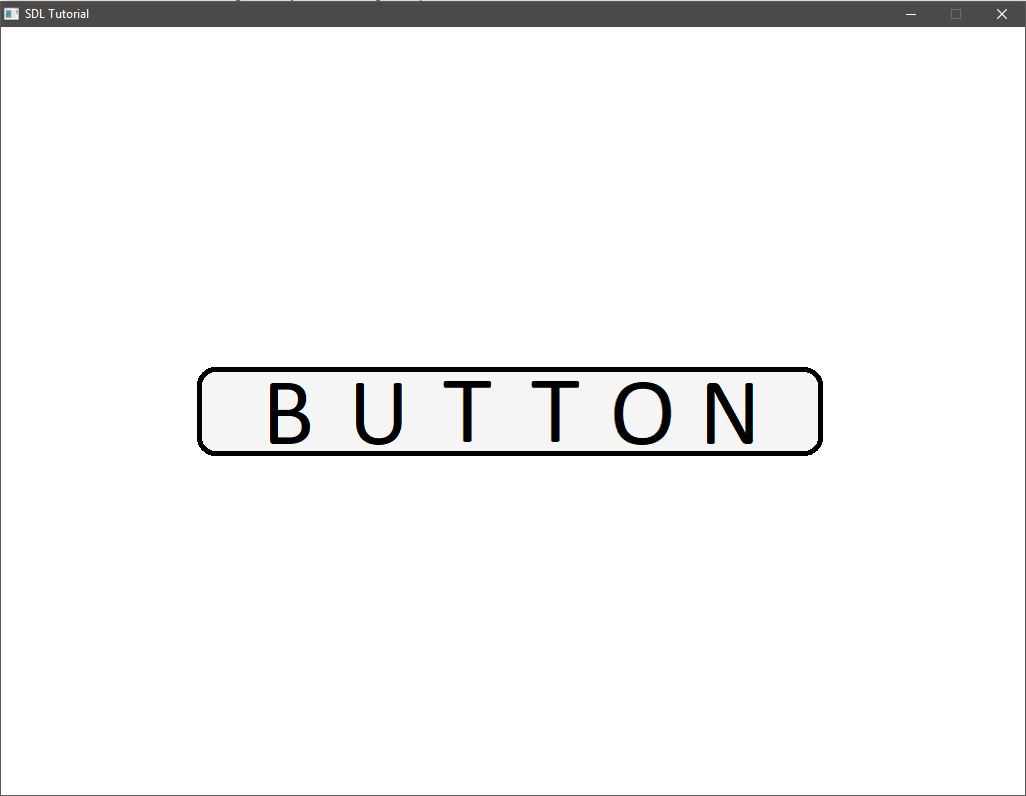
\includegraphics[scale=0.38]{screen.PNG}
  \caption{Output of the main() function}
\end{figure}

\newpage
\section{Problems}\index{Problems}

\begin{problem} Using the \texttt{SDL\_SetTextureAlphaMod()} Function, make Text appear and Disappear on the screen. You may have to create a new function in your LTexture Class to control Alpha (Opacity) of your Texture.\\
\end{problem}
\begin{problem} Make Text Slide from left to the center of screen when the Window opens. You may have to create a Move Function inside your Text Class and make it so that the Text moves by changing the Text Object's coordinates.\\
\end{problem}
\begin{problem} Modify your Button Class so that when you press it the Screen Background Color changes, and when you hover the cursor over the button its color changes from blue to green. For both the Button Press and Hover Animation, you have to check if the cursor coordinates fall inside the Button's coordinates.
\end{problem}

\newpage
\section{Solution}
\begin{lstlisting}[language=C++]
  // ... copy and paste your code
\end{lstlisting}

\newpage
\section{Student Feedback}\index{Student Feedback}
\textbf{What did you learn from this lab?}\\
\noindent\fbox{\parbox{\textwidth}{
    % Your feedback here.
  }
}\\
\textbf{What part of the lab is still unclear to you?}\\
\noindent\fbox{\parbox{\textwidth}{
    % Your feedback here.
  }
}\\
\textbf{What can be improved in this lab?}\\ 
\noindent\fbox{\parbox{\textwidth}{
    % Your feedback here.
  }
}


\end{document}


  
% \newpage
% % ----------------------------------------------------------------------------------------
% \chapterimage{chapter_head_2.pdf} % Chapter heading image
% \chapter{Constructors in C++ \hspace{36mm} {\textsc{\small SCRIPTED BY : MINHAJ AHMED}}}

% \section{Objective}\index{Objective}

% This Lab session introduces you to the Different types of Constructors in C++. In this lab, you will learn

% \begin{itemize}
% \item The different types of Constructors.
% \item Overloaded Constructors.
% \item Copy Constructors.
% \item Destructors
% \item Array of Pointers.
% \end{itemize}

% % ------------------------------------------------

% \section{Key Concepts}\index{Key Concepts}

% \subsection{Constructors}

% Constructors are special member functions of a class that are used for initializing Objects of that class. They are defined within the class and have the same name as the class. They are automatically called upon the creation of an object. Their return type is not specified in the code. If we don't specify a constructor, C++ generates a default constructor that doesn't take any parameters and has an empty body.

% \subsection{Constructor Overloading}

% Function Overloading is a concept in modern programming languages in which two functions may have the same name. The difference between the two functions having the same name is that they have different number, type or order of parameters, but all overloaded functions have the same return type. Like Function Overloading , Constructors can be overloaded too. By giving varying parameter types, we can make different Constructors. First of all, there are two types of constructors for an object. The \textbf{Default Constructor} (also known as the \textbf{Nullary} or \textbf{Parameterless} constructor) does not contain any parameter, and is called by default even if it is not defined by the programmer. The \textbf{Overload Constructor}, takes parameters and initializes the data members of the objects. According to the need, there can be multiple overloaded constructors.

% \subsection{Copy Constructors}

% Copy Constructors are a special type of overloaded constructors that initialize an object using another object, copying the other objects properties in the newly initialized object. The Copy Constructor takes an object by reference as its parameter, in order to access each of its data members and member functions, which can't be done when passing the object by value. Bear in mind that the object being passed in the copy constructor as the parameter must belong to the same class as the object being initialized. The \texttt{const} keyword is used to ensure that the object being passed doesn't get its properties changed in the copy constructor.

% % https://www.cs.nmsu.edu/~rth/cs/cs177/map/datamem.html

% \subsection{Destructors}

% Destructors are special member functions, just like Constructors, that are called automatically when the object goes out of scope or is explicitly deleted. They are used to deallocate memory and do other cleanup for a class object and its data members when the object is destroyed.


% \begin{lstlisting}[language=C++, caption={Declaration of Overloaded Constructors, Copy Constructor and Destructor}]
%   struct Light
%   {
%     bool activated;
%     int brightness;
    
%     Light();                                // Default Ctor
%     Light(bool activated);                  // Overloaded Ctor 1
%     Light(int brightness);                  // Overloaded Ctor 2
%     Light(bool activated, int brightness);  // Overloaded Ctor 3
%     Light(const Light& light);              // Copy Ctor
%     ~Light()                                // Destructor
%   }
% \end{lstlisting}

% \subsection{Array of Pointers}

% Just like how we can declare an array of integers, characters, or strings or user-defined objects, we can also declare an array of pointers that can point to different objects of the same type, for example, an array of integer pointers will have each of its entries point to integers. We can also declare a dynamic array of pointers. Each of its elements are empty pointers when the array is made. Each of these pointers can be used for dynamic memory allocation for objects or can point to already created objects. Deleting an array of pointers might involve accessing each of its elements and deleting them individually as each of its elements are pointers to objects. In the code on the next page, \texttt{lights} is a static array of pointers, while lightptrs is a dynamic array of pointers. Detailed usage is under the Syntax Examples.
% \vfill

% \begin{lstlisting}[language=C++, caption=Declaration of Arrays of Pointers]
%   int main()
%   {
%     Light *lights[4];   // Static Array of Pointers to 10 integers
%     Light **lightptrs;  // Declaration of Pointer to a Pointer
%     // Initialization of the Dynamic Array of Pointers
%     lightptrs = new Light*[4];
%     for (int i = 0; i < 4; i++)
%     {
%       lights[i] = new Light(); // Filling the Static Array
%       lightptrs[i] = new Light(); // Filling the Dynamic Array
%     }
%   }
% \end{lstlisting}

% % ------------------------------------------------
% % \vspace{-1.3cm}

% \section{Syntax Examples}\index{Syntax Examples}

% % \vspace{-1em}

% \begin{lstlisting}[language=C++, caption={Default, Overloaded and Copy Constructors}]
%   struct BookShelf
%   {
%     int capacity;
%     Book** books;
%     int noOfBooks;
%     BookShelf()
%     {   // Default Constructor
%       noOfBooks = 0;
%     }
%     BookShelf(int Bookcapacity)
%     {   // Overloaded Constructor
%       this->capacity = Bookcapacity;
%       books = new Book*[capacity];
%       noOfBooks = 0;
%     }
%     BookShelf(const BookShelf& bookshelf) 
%     {   // Copy Constructor
%       this->capacity = bookshelf.capacity;
%       this->noOfBooks = bookshelf.noOfBooks;
%       this->books = bookshelf.books;
%     }
%     Add(Book book)
%     {   // Member Function
%       if (noOfBooks < capacity)
%       {
%         this->books[noOfBooks] = book;
%         noOfBooks++;
%       }
%     }
%     ~BookShelf()                            
%     {   // Destructor
%       delete [] books;
%     }
%   }
% \end{lstlisting}


% % Notice that we didn't make any destructor in our class. That doesn't mean the class does not have any destructor at all. The compiler generates a destructor for the class just like it generates a default constructor. When do we define a destructor for our class then?  When we dynamically allocate any memory using a pointer, we need to free that memory in our destructor, since the automatically generated destructor only deletes the objects, and doesn't free any dynamically allocated memory. The code below doesn't contain any dynamically allocated memory (objects made by \texttt{new} keyword). Also, 

% Even if we don't define our destructor for our class, the compiler generates one for us, that deallocates all objects made inside the class, but it cannot deallocate any dynamically allocated memory, i.e objects created with the \texttt{new} keyword. For such objects we have to define our own destructor which deallocates all dynamically allocated objects.


% % \begin{lstlisting}[language=C++, caption={Use of Array of Pointers and Destructors}]
% %   struct Car
% %   {
% %   String model;
% %   String registration;
% %   Person* passengers;

% %   Car()                           // Default Ctor
% %   {
% %   model = "";
% %   registration = "";
% % }
% %   // Overloaded Constructor
% %   Car(String Model, String Registration, Person[] persons)
% %   {
% %   this->model = Model;
% %   this->registration = Registration;
% %   this->passengers = persons;
% % }
% %   Car(const Car& car)   // Copy Constructor
% %   {
% %   this->model = car.model;
% %   this->registration = car.registration;
% %   this->passengers = car.passengers;
% % }
% %   // passengers can exist outside of the car object, so
% %   // the pointers to the passengers will be made NULL,
% %   // rather than deleting them in the Destructor.
% %   ~Car()               // Destructor
% %   {
% %   for (int i = 0; i < 4; i++)
% %   {
% %   this->passengers[i] = NULL;
% % }
% % }
% % }
% % \end{lstlisting}

% \begin{lstlisting}[language=C++, caption={Use of Array of Pointers and Destructors}]
%   int main()
%   {
%     int** ptrs;                 //Pointer to an array of pointers
%     ptrs = new int*[5];         // Dynamic allocation of array of 
%     for (int i = 0; i < 5; i++) // pointers
%     {
%       ptrs[i] = new int(i);   // making new objects in each 
%     }                           // element of the pointer array.
%     for (int i = 0; i < 5; i++)
%     {
%       cout << *(ptrs[i]);     // Each entry is a pointer, for the
%     }                           // value we need to dereference it.
%     for (int i = 0; i < 5; i++)
%     {
%       delete ptrs[i];         // Delete each pointer
%     }  
%     delete [] ptrs;             // Delete the pointer array
    
%     return 0;
%   }
% \end{lstlisting}

% \newpage
% \section{Problems}\index{Problems}

% \begin{problem} Make a class Point which has x and y coordinates as its data members, and a display() member function that shows the coordinates in the format (x,y) on the console. Make its default, overloaded and copy constructors. \\
% \end{problem}
% \begin{problem} Write a Class Quadrilateral that has an array of pointers that points to 4 Objects of type Point. Make its default, overloaded and copy constructors and destructor. There must be an overload constructor that takes coordinates in integer type, an overloaded constructor that takes 4 Point Objects and copies them to create new objects. Remember that dynamically created objects have to be deleted explicitly. \\
% \end{problem}
% \begin{problem} Write a C++ Class called SuperString that contains a character array pointer as an attribute. Make its default, overloaded and copy constructors and destructor. The Overloaded Constructor must take a char array as an argument. The class must have a display() that prints the text on the console, an empty() function that empties the SuperString, and a length() function that returns the length of the SuperString. All these functions have to be member functions of the class.
% \end{problem}

% \newpage
% \section{Solution}
% \begin{lstlisting}[language=C++]
%   // ... copy and paste your code
% \end{lstlisting}

% \newpage
% \section{Student Feedback}
% \textbf{What did you learn from this lab?}\\
% \noindent\fbox{\parbox{\textwidth}{
%     % Your feedback here.
%   }
% }\\
% \textbf{What part of the lab is still unclear to you?}\\
% \noindent\fbox{\parbox{\textwidth}{
%     % Your feedback here.
%   }
% }\\
% \textbf{What can be improved in this lab?}\\ 
% \noindent\fbox{\parbox{\textwidth}{
%     % Your feedback here.
%   }
% }\\

% \newpage
% % ----------------------------------------------------------------------------------------
% \chapterimage{chapter_head_2.pdf} % Chapter heading image

% \chapter{More On Constructors \hspace{32mm} {\textsc{\small SCRIPTED BY : ABDUL RAFAY}}}
% \section{Default Constructor}\index{Default Constructor} 
% Default constructors initializes the class internals.It is created by compiler by default if user has not declared a constructor and they are called automatically when an object is made.

% \subsection{Sample Code}
% \begin{lstlisting}
%   class myClass
%   {
%     public:
%     myClass()
%     {
%       health = 100;
%       daysOfWeek = 7;
%       cout << "Default Constructor called" << endl;
%     }
    
%     private:
%     int health;
%     int daysOfWeek;
%   };
  
%   void main()
%   {
%     myClass obj;
%   }
% \end{lstlisting}
% \textbf{Output:} \\
% Default Constructor called\\

% \section{Constructor Overloading}\index{Constructor Overloading}
% Constructors can be overloaded the same way function are overloaded in c++.Overloaded constructors have the same name as the class and they vary in terms of number and types of arguments passed: upon which a specific constructor is called.

% \subsection{Sample Code}
% \begin{lstlisting}
%   class myClass
%   {
%     public:
%     myClass(int HEALTH, int DOW)
%     {
%       health = HEALTH;
%       daysOfWeek = DOW;
%     }
%     private:
%     int health;
%     int daysOfWeek;
%   };
  
%   void main()
%   {
%     //Overload constructor with 2 int type arguments is called
%     myClass obj(100, 7);  
%   }
% \end{lstlisting}
% \subsection{Copy Constructor}\index{Copy Constructor}
% There is a special type of overloaded constructor called the 'Copy Constructor' which takes reference of an object of the same class and copies the content of the referenced object into the object whose copy constructor is called.
% \subsection{Sample Code}
% \begin{lstlisting}
%   class myClass
%   {
%     public:
%     myClass(const myClass& ref_obj)
%     {
%       health = ref_obj.health;
%       daysOfWeek = ref_obj.daysOfWeek;
%     }
%     private:
%     int health;
%     int daysOfWeek;
%   };
  
%   void main()
%   {
%     /*
%     Copy constructor is called when an object is assigned to another object 
%     of the same class
%     */
    
%     myClass ref_obj(100, 7);
%     myClass obj = ref_obj; //Copy Constructor called
%   }
% \end{lstlisting}
% \begin{tcolorbox}[width=\textwidth,colback={white},title={KEYNOTE},colbacktitle=purple!50!white,coltitle=black]
%   By design all the private variables are per class and \emph{NOT}  per object that is why objects of same class can have access to each others private variable. Due to this reason in listing shown above health = \texttt{ref\_obj}.health does not give any error.
  
% \end{tcolorbox}

% \section{Problems}\index{Problems}
% You are going to Write your own String class. Let us call it SuperString
% The class will have constructor, overloaded constructor that takes in a \emph{character array}, destructor, copy constructor
% It will have a character array pointer as an attribute.
% It will have the following functions:\\
% \begin{enumerate}
% \item Join FUNCTION that takes in 2 CHARACTER ARRAYS and joins them together and returns a longer SuperString
% \item An overloaded Join FUNCTION that takes in two SuperStrings and joins them together and returns a longer SuperString
% \item Slice function that takes the starting index and ending index and returns a sliced SuperString.
% \item Show function that shows the SuperString
% \item Empty that empties the SuperStrin g.
% \item LENGTH THAT RETURNS THE LENGTH OF THE SuperString
% \end{enumerate}
% \hfill \break
% Start from defining the Constructors and Destructor!

% \subsection{Sample Code}
% \begin{lstlisting}
%   #include <iostream>
  
%   using namespace std;
  
%   class SuperString
%   {
%     private:
%     char* text;
%     int length;
%     public:
%     SuperString()
%     {
%       length = 0;
%       text = NULL;
%     }
%     SuperString(char* txt)
%     {
%       /*
%       Step 1: Calculate length of the character array
%       Step 2: Allocate Dynamic memory to store the characters of
%       passed array into text pointer of class
      
%       Note 1: Since elements in the array are stored in sequential
%       order in memory,therefore,a pointer storing address of the
%       first element of the array can simple increment the address by 
%       1 to access the next element of the array and so on.Name of any 
%       array is actually the name of the pointer pointing at the first
%       element of the array. For example:
%       " char array[10] ",'array' is a character type pointer pointing
%       at element at the 0 index of the array.
%       In this task we will not increment the pointer
%       however c++ gives us the functionality to access all the
%       elements in array using indexing for example array[2] refers to
%       the element at the 2nd index of array.
      
%       Note 2: All character end must have their last element as 
%       character or NULL '\0' known as the NULL terminator.This
%       indicates the end of a string or character array.
      
%       */
%     }
%     SuperString(const SuperString& myString)
%     {
%       /*
%       Shallow copy is when two collections share the 
%       individual elements.Changes made to the elements
%       of any collections will change both collections
%       Deep copy of a collection is when elements of a 
%       collections is copied to the other collection. Both
%       these collections work independently once
%       the elements are copied unlike shallow
%       copy.
      
%       Note 1: Parameter of this function is a constant 
%       which means function must not change the input object
%       while making a copy. (Hint: make deep copy) 
%       */
%     }
    
%     void Show()
%     {
%       //Displays text
%     }
    
%     SuperString Join (char array_1[], char array_2[])
%     {
%       /*
%       Step 1: Calculate length of both the arrays
%       and create a dynamic array whose length is the
%       sum of the length of array_1 and array_2 
%       Step 2: Copy the elements of both the arrays
%       into the new array created.
%       Step 3: Pass the new array to a SuperString
%       object and return the object
%       */
%       int len_array_1 = 0;
%       int len_array_2 = 0;
      
%       //Write your code here
      
%       int tempLen = len_array_1 + len_array_2;
%       char* temp = new char[tempLen+1];
%       //+ 1 is done to store NULL terminator
%       //Write your code here
%     }
    
%     SuperString Join (SuperString& a,SuperString& b)
%     {
%       //Write your code here
%     }
    
%     SuperString Slice(int start, int end){}
%     SuperString Empty(){}
%     ~SuperString(){}
    
%   };
% \end{lstlisting}

% \newpage
% \section{Solution}
% \begin{lstlisting}[language=C++]
%   // ... copy and paste your code
% \end{lstlisting}

% \newpage
% \section{Student Feedback}
% \textbf{What did you learn from this lab?}\\
% \noindent\fbox{\parbox{\textwidth}{
%     % Your feedback here.
%   }
% }\\
% \textbf{What part of the lab is still unclear to you?}\\
% \noindent\fbox{\parbox{\textwidth}{
%     % Your feedback here.
%   }
% }\\
% \textbf{What can be improved in this lab?}\\ 
% \noindent\fbox{\parbox{\textwidth}{
%     % Your feedback here.
%   }
% }\\


% \newpage
% \chapterimage{chapter_head_2.pdf} % Chapter heading image
% \chapter{Double-linked list \hspace{40mm} {\textsc{\small SCRIPTED BY : HAMZA MASROOR}}}
% \section{Objective}\index{Objective}
% In this lab, we'll learn about a data structure, called Double linked list. We'll learn about its implementation, operations and uses.
% \section{Description}\index{Description}
% Double linked list is a sequence of elements in which every element has links to its previous element and next element in the sequence.
% It has the same operations as the single-linked list, but the operations takes less time as there are shorter traversals using links to both next and previous element. We'll see it in the examples below.

% \subsection{Real-life examples of Double linked list}
% There are many real life examples of stack. Consider the simple example of a music player. The music player allows skipping to both next and previous song in the playlist. Moreover, it allows to traverse through the list to find a song using both next and previous buttons.

% \subsection{Time Complexities of Double linked list}
% Append(data) - O(1) time \\
% Add(i, data) - O(min(i, n - i))\\
% Remove(i) - O(min(i, n - i))\\ 
% Where i is the index and n is the size of the list.\\ \\
% For add and remove, we have to find the node at the index where a node is getting added or removed. Finding the node with a particular index in a DLList is easy; we can either start at the head of the list and work forward ,or start at the tail of the list and work backward. This allows us to reach the ith node in O(min(i,n - i)) time.

% \subsection{Applications of Double linked list}
% There are many possible applications of stack. Some are listed below:
% \begin{itemize}
% \item The browser cache which allows you to hit the BACK buttons (a linked list of URLs).
% \item Applications that have a Most Recently Used (MRU) list (a linked list of file names).
% \item A stack, hash table, and binary tree can be implemented using a doubly linked list. 
% \item Undo functionality in Photoshop or Word (a linked list of state).
% \end{itemize}

% \section{Implementation}
% We will be implementing a double linked list. In double linked list, we have nodes linked to each other.
% Each node stores a data and links to the node next to and previous to it.
% \begin{figure}[H]
%   \centering
%   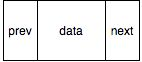
\includegraphics{DLNode.jpeg}
%   \caption{Representation of node}
% \end{figure}
% \paragraph{Implementing Node}
% To implement node, we will be making a struct to hold data and the links to store next and previous node . In this implementation we are making a node to store integer type data. However, it can be implemented to store any data type or object.
% \begin{lstlisting}
%   struct Node
%   {
%     int data;
%     Node* next;
%     Node* prev;
%     Node()
%     {
%       next = NULL;
%       prev = NULL;
%     }
%   };
% \end{lstlisting}
% \paragraph{Initializing the Double linked list}
% As a Double linked consists of many nodes, we should have many nodes inside our DLList class, but we will have only two nodes, "head" and "tail", which will act as reference nodes and allows us to iterate through all the nodes in the DLList. Moreover, we will include an integer "length" to keep track of the size of the list.
% \begin{lstlisting}
%   class DLList
%   {
%     private:
%     int length;
%     Node* head;
%     Node* tail;
%     public:
%     DLList()
%     {
%       head = NULL;
%       tail = NULL:
%     }
%   }
% \end{lstlisting}
% Our stack now consists of Node pointers which will hold the addresses of the head and the tail. To initialize, both are set to \textbf{NULL}, as the list is empty.
% \begin{figure}[H]
%   \centering
%   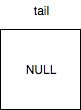
\includegraphics{DLList1.jpeg}
%   \caption{DLList head pointer}
% \end{figure}
% \begin{figure}[H]
%   \centering
%   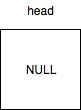
\includegraphics{DLList2.jpeg}
%   \caption{DLList tail pointer}
% \end{figure}
% \paragraph{Implementing Append operation}
% Inside the class of DLList, we will declare and define a function "Append(int data)" in public.
% \begin{lstlisting}
%   void Append(int data)
%   {
%     if (length == 0)
%     {
%       head = tail = new Node();
%       head->data = data;
%     }
%     else
%     {
%       tail->next = new Node();
%       tail->next->prev = tail;
%       tail = tail->next;
%       tail->data = data;
%     }
%     length++;
%   }

% \end{lstlisting}
% \begin{example}
%   Let's visualize an example Append() operation\\
%   \begin{lstlisting}
%     DLList lst;
%     lst.Append(6);
%   \end{lstlisting}
%   Since the DLList is empty and head is set to NULL. Body of 'if' will be executed.\\
%   It first creates a new node and sets head and tail to it.\\
%   \begin{figure}[H]
%     \centering
%     \includegraphics[scale=0.5]{DLList3.jpeg}
%     \caption{Creating new node}
%   \end{figure}
%   ~\\
%   Then it sets its data to the data passed.
%   \begin{figure}[H]
%     \centering
%     \includegraphics[scale=0.5]{DLList5-set.jpeg}
%     \caption{Setting data}
%   \end{figure}
% \end{example}
% Since, length is not '0', Append operation will now execute body of 'else'. Let's see an example
% \begin{example}
%   \begin{lstlisting}
%     lst.append(9);
%   \end{lstlisting}
%   It will first create a new node and sets tail's next to it.
%   \begin{figure}[H]
%     \centering
%     \includegraphics[scale=0.5]{DLList4.jpeg}
%     \caption{Creating new node}
%   \end{figure} ~\\
%   Then it sets the new node's prev to the tail
%   \begin{figure}[H]
%     \centering
%     \includegraphics[scale=0.5]{DLList5.jpeg}
%     \caption{Setting new node's pointer}
%   \end{figure}
%   It now updates the tail and sets data.
%   \begin{figure}[H]
%     \centering
%     \includegraphics[scale=0.5]{DLList6.jpeg}
%     \caption{Updating tail and data}
%   \end{figure}
%   '9' is added succesfully.
%   {\begin{figure}[H]
%       \centering
%       \includegraphics[scale=0.5]{DLList7.jpeg}
%       \caption{Succesful Append(9) operation}
%     \end{figure}}
% \end{example}

% \paragraph{Implementing Add operation}
% Inside the class of DLList, we will declare and define a function "Append(int data)" in public.
% \begin{lstlisting}
%   void Add(int i, int data)
%   {
%     if(i >= 0 && i <= length)
%     {
%       if (i == 0)
%       {
%         if (length == 0)
%         {
%           head = tail = new Node();
%           head->data = data;
%         }
%         else
%         {
%           head->prev = new Node;
%           head->prev->next = head;
%           head = head->prev;
%           head->data = data;
%         }
        
%       }
%       else if (i == length)
%       {
%         tail->next = new Node();
%         tail->next->prev = tail;
%         tail = tail->next;
%         tail->data = data;
%       }
%       else
%       {
%         Node* temp;
%         if (i <= length/2)
%         {
%           temp = head;
%           for (int j = 0; j < i; j++)
%           {
%             temp=temp->next;
%           }
%         }	
%         else
%         {
%           temp = tail;
%           for (int j = 0; j < length-i-1; j++)
%           {
%             temp = temp->prev;
%           }
%         }
        
%         Node* newNode = new Node;
%         newNode->data = data;
%         newNode->prev = temp->prev;
%         newNode->next = temp;
%         temp->prev->next = newNode;
%         temp->prev = newNode;
        
%       }
%       length++;
%     }
%     else
%     {
%       cout << "Index is out of range" << endl;
%     }
%   }

% \end{lstlisting}
% \begin{example}
%   Let's visualize an example Add() operation\\
%   \begin{lstlisting}
%     DLList lst;
%     lst.Add(0,6);
%   \end{lstlisting}
%   Since the DLList is empty, Body of 'if (i == 0) and if (length == 0)' will be executed.\\
%   It will carry out the same operations carried out in Append function.\\
%   It first creates a new node and sets head and tail to it.\\
%   \begin{figure}[H]
%     \centering
%     \includegraphics[scale=0.5]{DLList3.jpeg}
%     \caption{Creating new node}
%   \end{figure}
%   ~\\
%   Then it sets its data to the data passed.
%   \begin{figure}[H]
%     \centering
%     \includegraphics[scale=0.5]{DLList5-set.jpeg}
%     \caption{Setting data}
%   \end{figure}
% \end{example}
% If a number is added to the last, it will then also do the same tasks as append.\\

% \begin{example}
%   \begin{lstlisting}
%     lst.Add(1,9);
%   \end{lstlisting}
%   Now length is not 0 and index is equal to the length.\\
%   It will first create a new node and sets tail's next to it.
%   \begin{figure}[H]
%     \centering
%     \includegraphics[scale=0.5]{DLList4-add.jpg}
%     \caption{Creating new node}
%   \end{figure} ~\\
%   Then it sets the new node's prev to the tail
%   \begin{figure}[H]
%     \centering
%     \includegraphics[scale=0.5]{DLList5-add.jpg}
%     \caption{Setting new node's pointer}
%   \end{figure}
%   It now updates the tail and sets data.
%   \begin{figure}[H]
%     \centering
%     \includegraphics[scale=0.5]{DLList6-add.jpg}
%     \caption{Updating tail and data}
%   \end{figure}
%   '9' is added succesfully.
%   {\begin{figure}[H]
%       \centering
%       \includegraphics[scale=0.5]{DLList7-add.jpg}
%       \caption{Succesful Add(1,9) operation}
%     \end{figure}}
% \end{example}
% \begin{example}
%   Let's look at an example, when index is neither 0 nor equal to the length.
%   Let's visualize an example Add() operation\\
%   \begin{lstlisting}
%     lst.Add(1,5);
%   \end{lstlisting}
%   Since i is less than half of the length, it will iterate from the head.\\
%   It will first create a temporary pointer and point it to head.
%   \begin{figure}[H]
%     \centering
%     \includegraphics[scale=0.5]{DLAdd1.jpg}
%     \caption{Creating a temporary pointer}
%   \end{figure} ~\\
%   It will iterate till it reaches the index where a new node is to be added.
%   \begin{figure}[H]
%     \centering
%     \includegraphics[scale=0.5]{DLAdd2.jpg}
%     \caption{Iterating till it reaches the node}
%   \end{figure}
%   It will create a new Node.
%   \begin{figure}[H]
%     \centering
%     \includegraphics[scale=0.5]{DLAdd3.jpg}
%     \caption{Creating new node}
%   \end{figure}
%   Points its 'prev' pointer to the temp's 'prev'.
%   \begin{figure}[H]
%     \centering
%     \includegraphics[scale=0.5]{DLAdd4.jpg}
%     \caption{Setting node's prev pointer}
%   \end{figure}~\\
%   Points its 'next' pointer to temp.
%   \begin{figure}[H]
%     \centering
%     \includegraphics[scale=0.5]{DLAdd5.jpg}
%     \caption{Setting node's next pointer}
%   \end{figure}
%   Point Node's prev's next pointer to itself.
%   \begin{figure}[H]
%     \centering
%     \includegraphics[scale=0.5]{DLAdd5(1).jpg}
%     \caption{Setting the previous node's next pointer}
%   \end{figure}
%   And finally temp's prev to the new node.
%   \begin{figure}[H]
%     \centering
%     \includegraphics[scale=0.5]{DLAdd6.jpg}
%     \caption{Succesful addition}
%   \end{figure}
% \end{example}
% \begin{example}
%   Now, let's see an example where index is greater than the half of the length of the list.\\
%   \begin{lstlisting}
%     lst.Add(2,13);
%   \end{lstlisting}
%   Since index is greater than the half of the length, it will start iteration from the last.\\
%   It will first create a temporary pointer and sets it to the tail.
%   \begin{figure}[H]
%     \centering
%     \includegraphics[scale=0.5]{DLAdd7.jpg}
%     \caption{Creating a temporary pointer}
%   \end{figure}
%   It will iterate till it reaches the index where the new node has to be added
%   \begin{figure}[H]
%     \centering
%     \includegraphics[scale=0.5]{DLAdd8.jpg}
%     \caption{Iterated till the index}
%   \end{figure}
%   Now it repeats the same process of setting pointers as it did above and adds the new node succesfully.
%   \begin{figure}[H]
%     \centering
%     \includegraphics[scale=0.5]{DLAdd10.jpg}
%     \caption{Succesful Add(2,13) operation}
%   \end{figure}
% \end{example}
% Let's see an example when the length is not '0' and the node is to be added at index '0'.
% \begin{example}
%   \begin{lstlisting}
%     lst.Add(0,4);
%   \end{lstlisting}
%   It will first create a new node and sets the prev's pointer, of the node pointed by head, to it.
%   \begin{figure}[H]
%     \centering
%     \includegraphics[scale=0.5]{DLAdd11.jpg}
%     \caption{Creating new node and setting head's prev}
%   \end{figure}~\\
%   Then it sets new node's next to the next of node pointed by head.
%   \begin{figure}[H]
%     \centering
%     \includegraphics[scale=0.5]{DLAdd12.jpg}
%     \caption{Setting node's next pointer}
%   \end{figure}~\\
%   Finally, head is set to the new node and the node is added succesfully.
%   \begin{figure}[H]
%     \centering
%     \includegraphics[scale=0.5]{DLAdd13.jpg}
%     \caption{Updating head}
%   \end{figure}
% \end{example}
% \paragraph{Implementing Show() function}
% The Show()  function allows to output all the values in the DLList. \\
% Inside the class of DLList, we will declare and define a function "void Show()" in public.
% \begin{lstlisting}
%   void Show()
%   {
%     Node* temp = head;
%     while(temp!=NULL)
%     {
%       std::cout<<temp->data<<std::endl;
%       temp = temp->next;
%     }
%   }
% \end{lstlisting}
% \newpage
% Let's visualize an example of Show() operation
% \begin{example}
%   \begin{lstlisting}
%     lst.Show();
%   \end{lstlisting}~\\
%   It creates a temp pointer and is pointed to the node pointed by head. It also outputs its value
%   \begin{figure}[H]
%     \centering
%     \includegraphics[scale=0.5]{DLShow1.jpg}
%     \caption{Creating temp pointer and outputting first value}
%   \end{figure} ~\\
%   It updates the temp pointer and moves to the next node. Then it outputs the value of the node pointed by temp.
%   \begin{figure}[H]
%     \centering
%     \includegraphics[scale=0.5]{DLShow2.jpg}
%     \caption{Outputting second value}
%   \end{figure}
%   \newpage
%   And finally it moves to the last node, outputs its value and since it's next is equal to NULL, the loop is ended.
%   \begin{figure}[H]
%     \centering
%     \includegraphics[scale=0.5]{DLShow3.jpg}
%     \caption{Outputting third value}
%   \end{figure} ~\\
% \end{example}
% \newpage
% \section{Problems}\index{Problems}
% \begin{problem}
%   Implement the Remove(int index) function in your DLList class. The function should remove the element from the given index and returns the removed element. The function should run in O(min(i, n - i)).
%   \paragraph{Instructions}
%   \begin{itemize}
%   \item Think for all special cases such as, removal at zero index and removal at last index.
%   \item Update pointers carefully.
%   \item Try to take an idea from given Add() function for traversal.
%   \end{itemize}
% \end{problem}
% ~\\
% \begin{problem}
%   Implement the function Reverse() which reverses the list, without making a new list.
%   \paragraph{Instructions}
%   \begin{itemize}
%   \item Traverse through the whole list and update its pointers accordingly
%   \end{itemize}
% \end{problem}

% \newpage
% \section{Solution}
% \begin{lstlisting}[language=C++]
%   // ... copy and paste your code
% \end{lstlisting}

% \newpage
% \section{Student Feedback}
% \textbf{What did you learn from this lab?}\\
% \noindent\fbox{\parbox{\textwidth}{
%     % Your feedback here.
%   }
% }\\
% \textbf{What part of the lab is still unclear to you?}\\
% \noindent\fbox{\parbox{\textwidth}{
%     % Your feedback here.
%   }
% }\\
% \textbf{What can be improved in this lab?}\\ 
% \noindent\fbox{\parbox{\textwidth}{
%     % Your feedback here.
%   }
% }
